% chktex-file 44
\documentclass[12pt]{article}
\usepackage[a4paper,margin=2cm]{geometry}
\usepackage{luatexja-fontspec}
\usepackage{setspace}
\usepackage{indentfirst}
\usepackage{graphicx}
\usepackage{amsmath}
\usepackage{amssymb}
\usepackage{booktabs}
\usepackage{threeparttable}
\usepackage{subcaption}
\usepackage{float}
\usepackage{pdfpages}
\usepackage{enumitem}
\usepackage{titlesec}
\usepackage{hyperref}
\usepackage{zhnumber}
\usepackage{graphbox}
\usepackage{array}

\setmainjfont[AutoFakeBold=2.5]{PMingLiU}


\setlength{\parindent}{2em}
\setlength{\parskip}{0pt}
\onehalfspacing%

\titleformat{\section}{\centering\bfseries\fontsize{16}{20}\selectfont}{}{0em}{}
\titleformat{\subsection}{\bfseries\fontsize{14}{18}\selectfont}{}{0em}{}
\titleformat{\subsubsection}{\bfseries\fontsize{12}{16}\selectfont}{}{0em}{}
\setcounter{secnumdepth}{0}

\author{翁浩庭、鄭沐臻}
\date{\today}

\begin{document}
\pagestyle{empty}
\pagestyle{empty} % 封面不顯示頁碼

\begin{center}
    \begin{spacing}{2.0}
        {\fontsize{20}{24}\selectfont \textbf{臺北市立建國高級中學 115 學年度科學展覽}} \\
        \vspace{0.3cm}
        {\fontsize{20}{24}\selectfont \textbf{作品說明書}} 
    \end{spacing}
    
    \vspace{4.5cm} 
    
    \begin{spacing}{2.0}
        {\fontsize{14}{18}\selectfont
        \begin{tabular}{l p{11cm}}
            \textbf{科\quad 別：} & 物理與天文學科 \\ 
            \textbf{組\quad 別：} & 高級中等學校組 \\ 
            \textbf{作品名稱：} & 聚苯乙烯微球懸浮液的多角度光散射 \\
                               & 與蒙地卡羅模擬 \\ 
            \textbf{關鍵詞：} & 微塑膠（microplastics）、光散射（light \\
                             & scattering）、蒙地卡羅模擬（Monte Carlo simulation） \\ 
            \textbf{編\quad 號：} &  \\ 
        \end{tabular}}
    \end{spacing}
    
\end{center}

\clearpage
\pagestyle{plain}
\pagenumbering{arabic}
\setcounter{page}{1}

\section*{摘要}
\subsection*{中文摘要}
本研究以氦氖雷射、TSL2591 光感模組與樂高自製多角度光強度測量裝置，
測量粒徑為 $2.16\mu m$ 與 $0.49\mu m$ 的聚苯乙烯微球在光學厚度
(Optical Thickness) $\tau$ 在 $0.5 \sim 8$ 之間時，
散射角 ${30}^{\circ }$與 ${125}^{\circ }$ 的光強度比值 $ C $ ，
並與蒙地卡羅模擬的結果作比較。結果顯示當粒徑相同時 $C$ 與 $\tau$ 呈現負相關，
當 $\tau$ 相同時，粒徑為 $2.16\mu m$ 的 $C$ 約為 $0.49\mu m$ 
的 $1.6\sim 2.4$ 倍，而模擬的結果亦與實驗結果具有相同趨勢。這顯
示多重散射下兩角度光強比仍保有粒徑資訊，且我們的模擬能有效預測
多重散射的趨勢。


\section*{壹、前言}
\subsection*{一、研究動機}
光散射（light scattering）法不需要前處理，元件也便宜，常用來分析水中微粒的大小，
例如微塑膠（microplastics）。多角度光散射利用不同角度的散射強度辨識粒徑，但多半在
稀薄的樣品中進行：此時光大多只被散射一次，角度分布就是單一粒子的散射圖形。樣品變濃
後，光會在樣品中被散射很多次（多重散射），方向逐漸被打亂，角度分布也跟著變平。我們
想知道：從單次散射過渡到多重散射時，散射光的角度分布會怎麼改變？兩個角度的強度比是
否仍與粒徑有關？蒙地卡羅模擬能否重現實驗的結果？

\subsection*{二、研究目的}
\begin{itemize}
    \item[(一)] 建立低成本的多角度光散射量測系統與數據處理流程。
    \item[(二)] 探討光學厚度 $\tau$ 對兩種粒徑（$0.49 \mu m$、$2.16 \mu m$）聚苯乙烯懸浮液兩角強度比 $C$ 的影響。
    \item[(三)] 比較實驗與蒙地卡羅模擬的結果。
\end{itemize}
\subsection*{三、文獻回顧}
已有研究指出，微塑膠的角度散射具有粒徑特徵（Genc et al., 2023），也有研究以多角度光散射辨識聚苯乙烯微球粒徑（Lotfi Choobbari et al., 2022）；然而，這些研究主要在稀薄、以單次散射為主的條件下進行。另一方面，蒙地卡羅模擬已用於描述聚苯乙烯懸浮液中的多重散射（Berrocal et al., 2007）。對於單次散射過渡至多重散射的區間，兩個角度的強度比如何隨光學厚度改變，尚未見直接相關研究。因此，本研究以兩角強度比作為指標，探討其在不同粒徑與光學厚度下的變化，並以蒙地卡羅模擬與實驗互相比較。


\section*{貳、研究設備及器材}
\subsection*{一、光學量測器材}
\begin{table}[H]
    \setlength{\extrarowheight}{1pt}
    \centering

    \begin{tabular}{|m{2cm}|m{3cm}|m{3cm}|m{3cm}|}
        \hline
        \centering 名稱 & \centering 氦氖雷射 & \centering TSL2591 感光元件 & \centering Arduino Uno  \tabularnewline \hline
        \centering 圖片 & 
        \centering 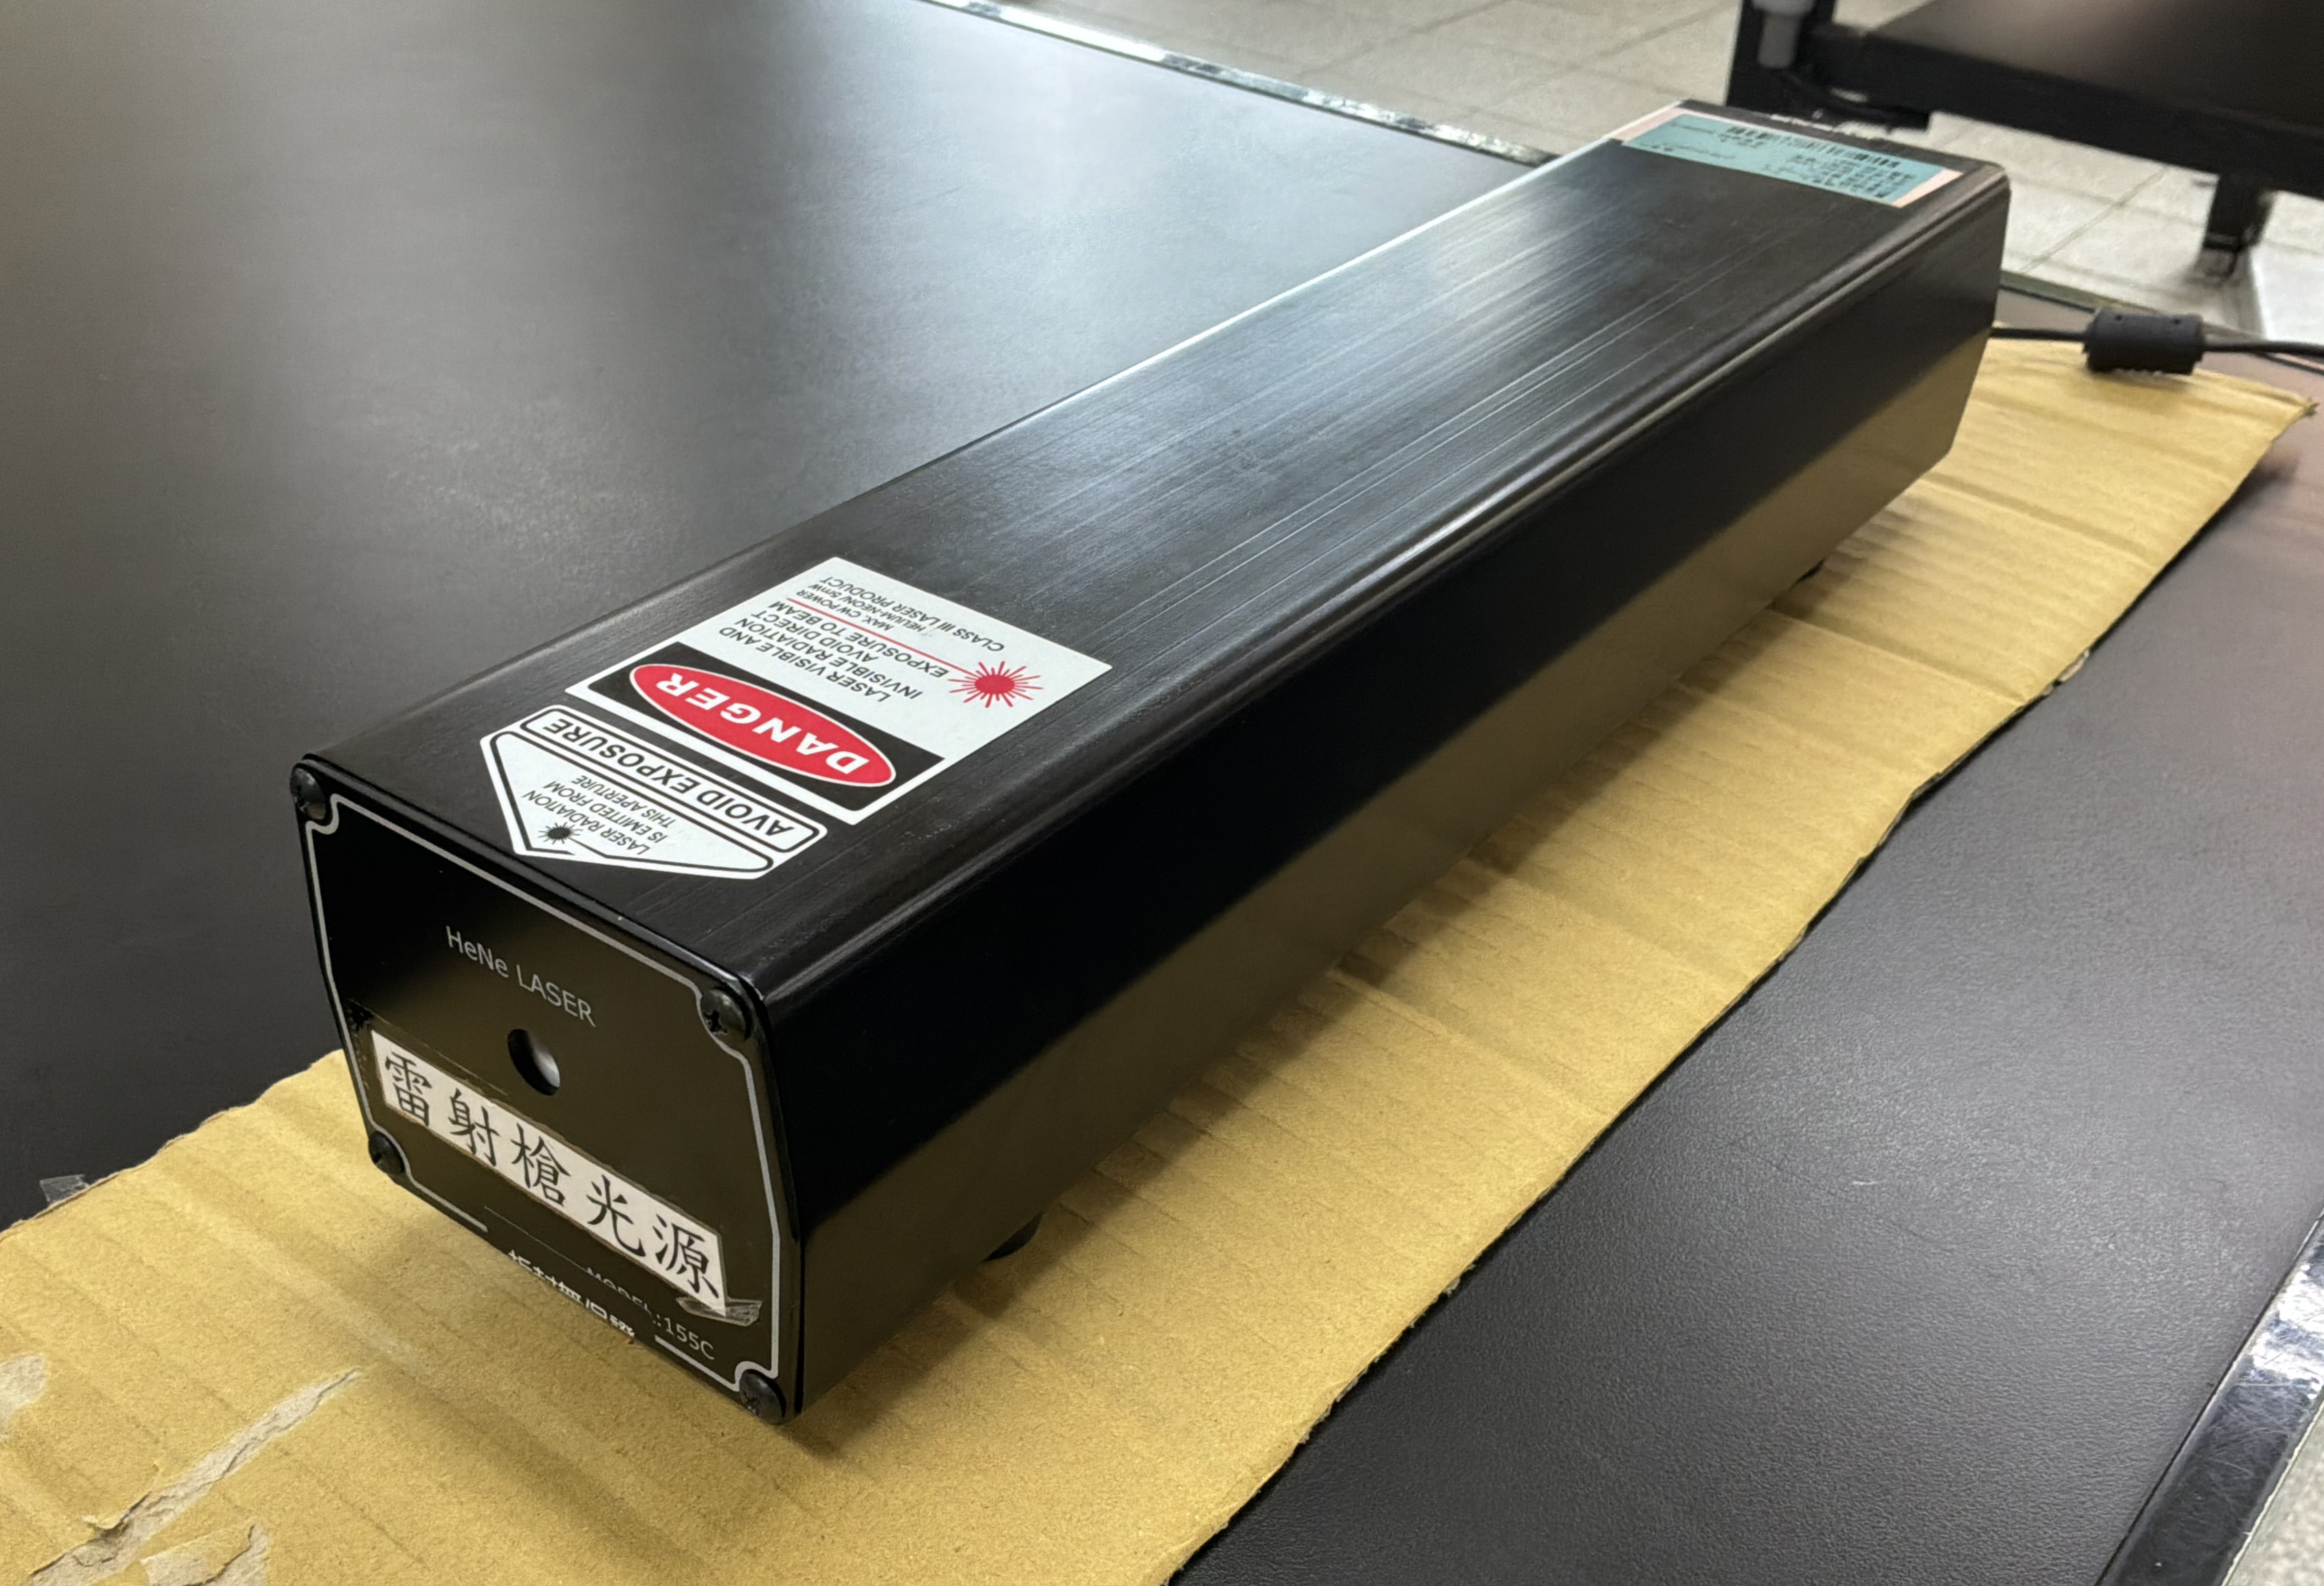
\includegraphics[width=3cm, align=c]{image/雷射槍.png} & 
        \centering 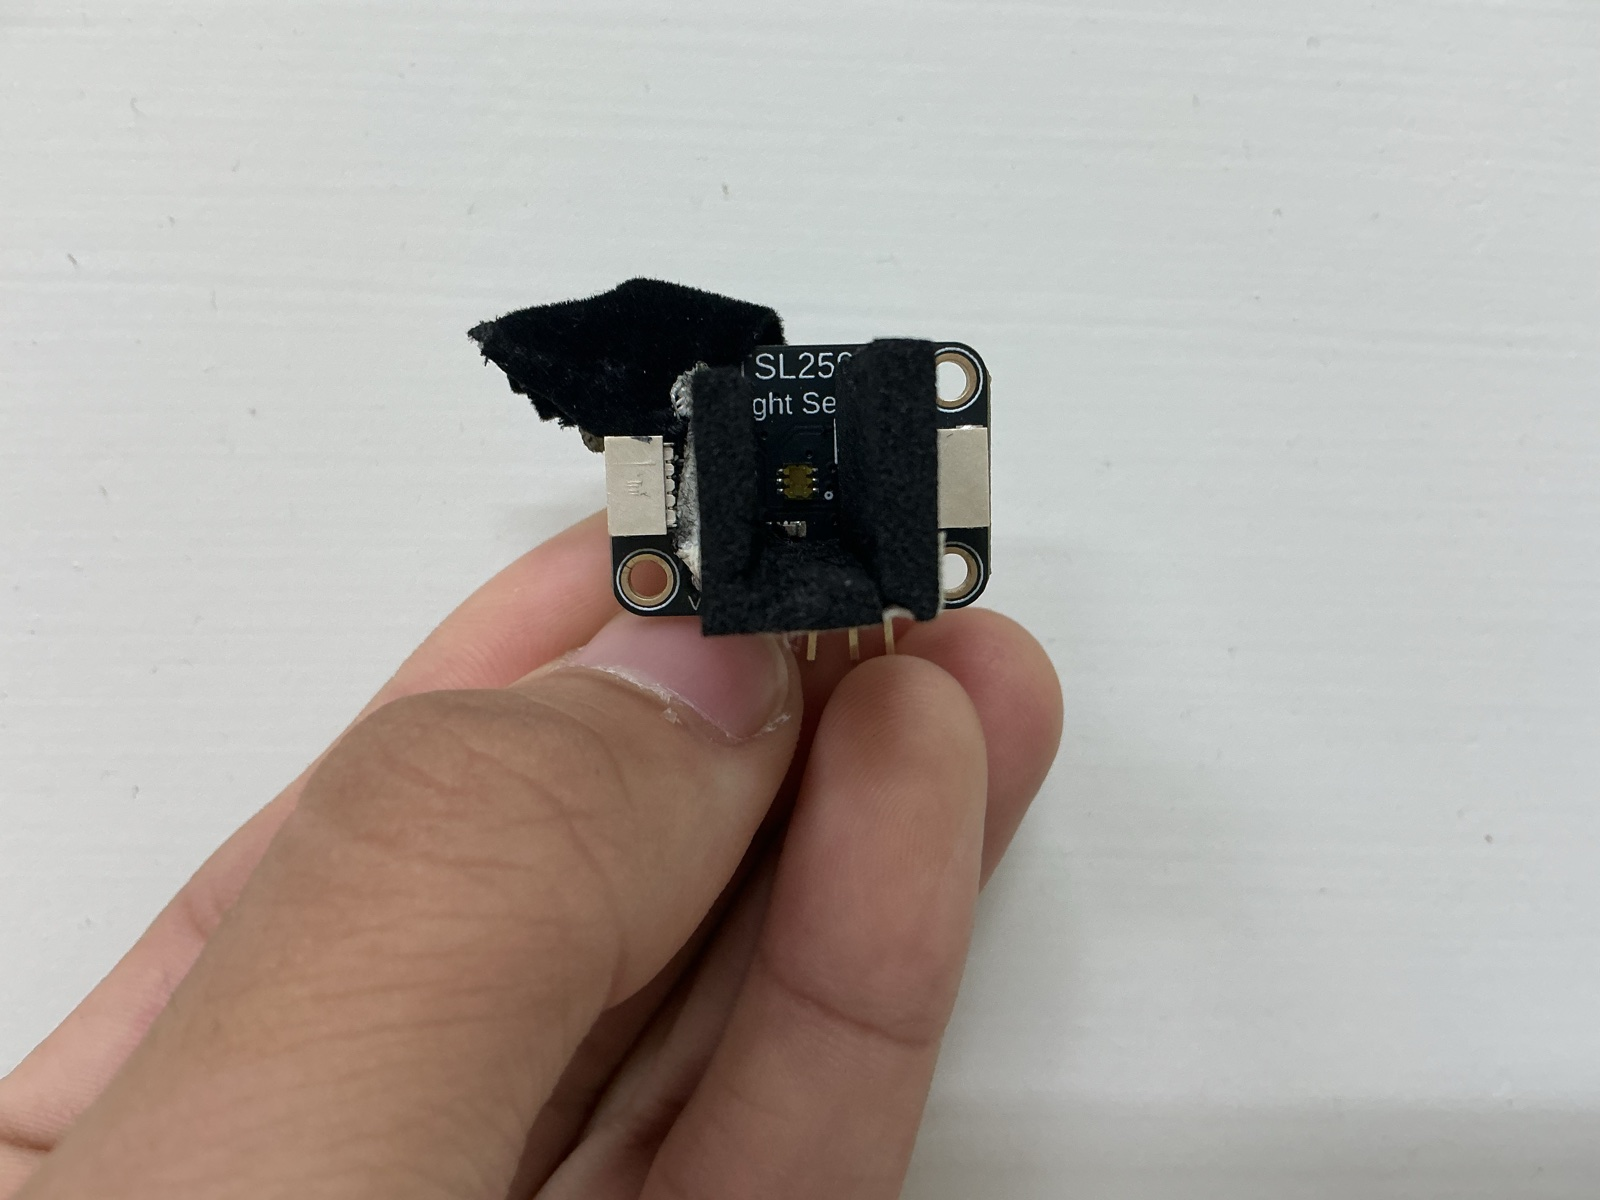
\includegraphics[width=3cm, align=c]{image/tsl2591.jpg} & 
        \centering 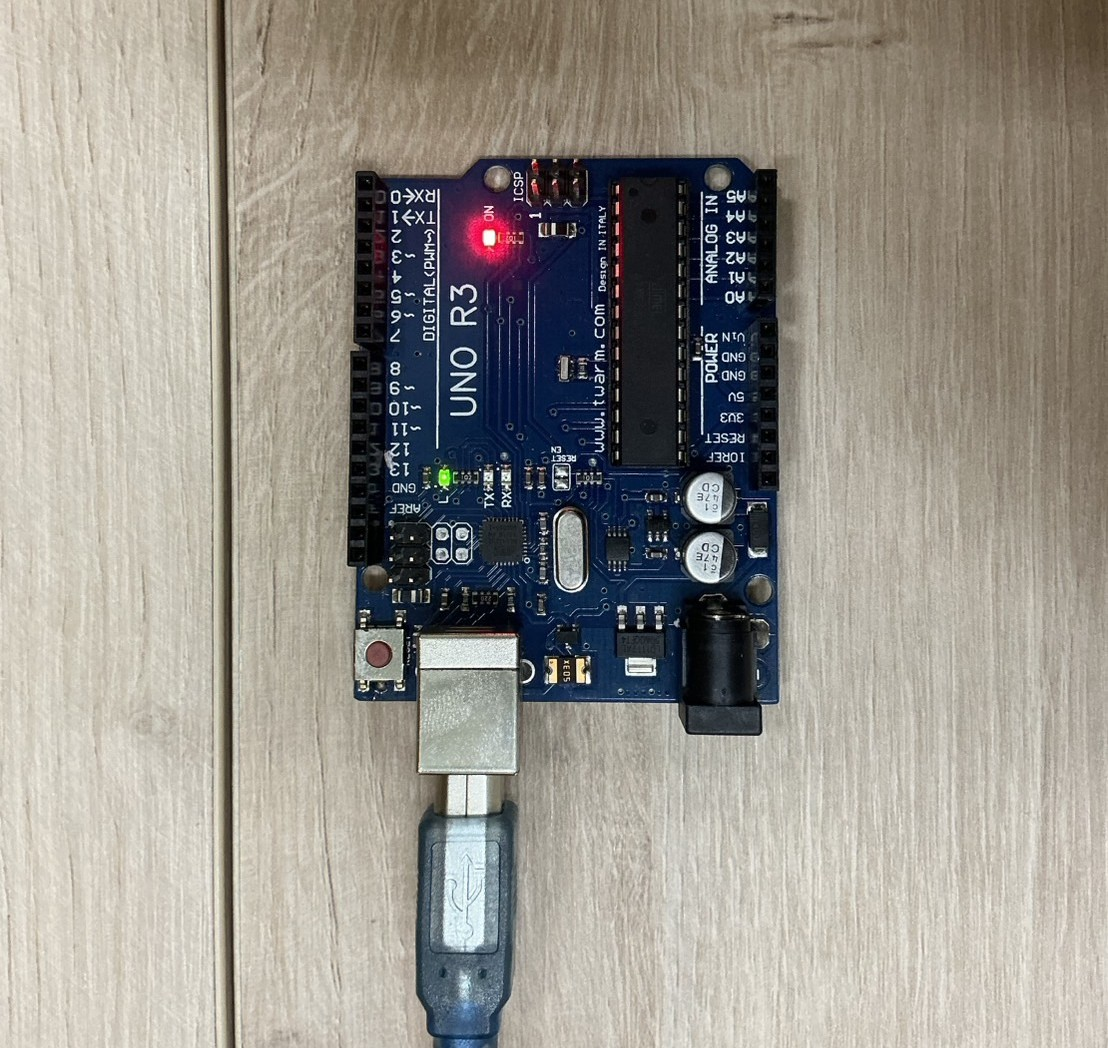
\includegraphics[width=3cm, align=c]{image/Arduino.JPG} \tabularnewline 
        \hline

        \centering 名稱 & \centering 旋轉臂 & \centering EV3 馬達模組 & 自動數據同步器  \tabularnewline 
        \hline
        \centering 圖片 & 
        \centering 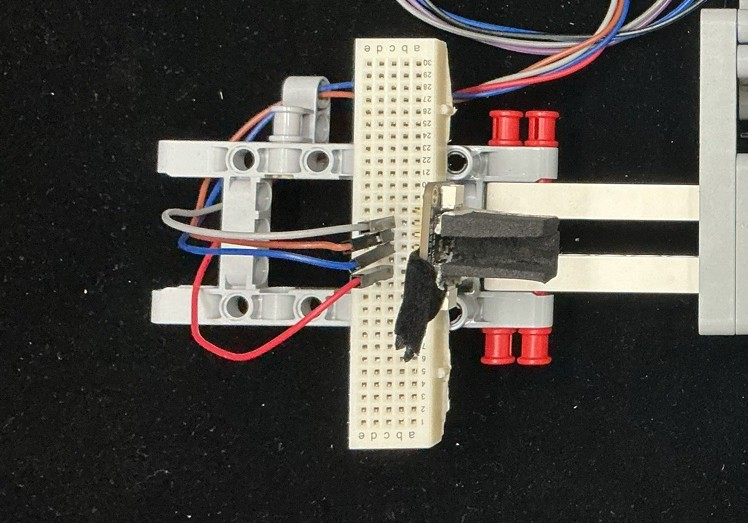
\includegraphics[width=3cm, align=c]{image/旋轉臂.jpg} & 
        \centering 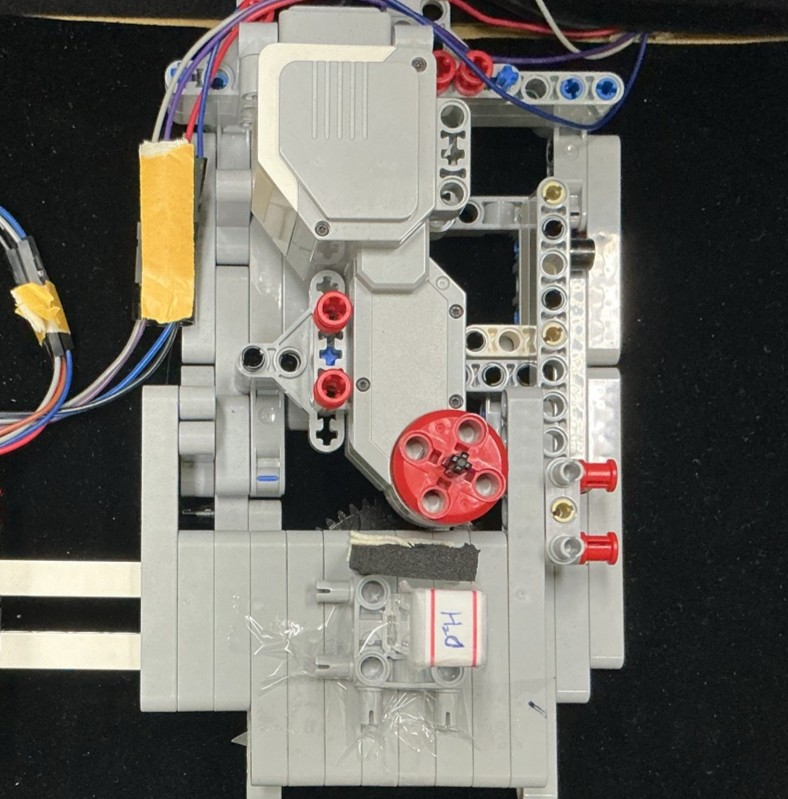
\includegraphics[width=3cm, align=c]{image/ev3.jpg} &
        \centering 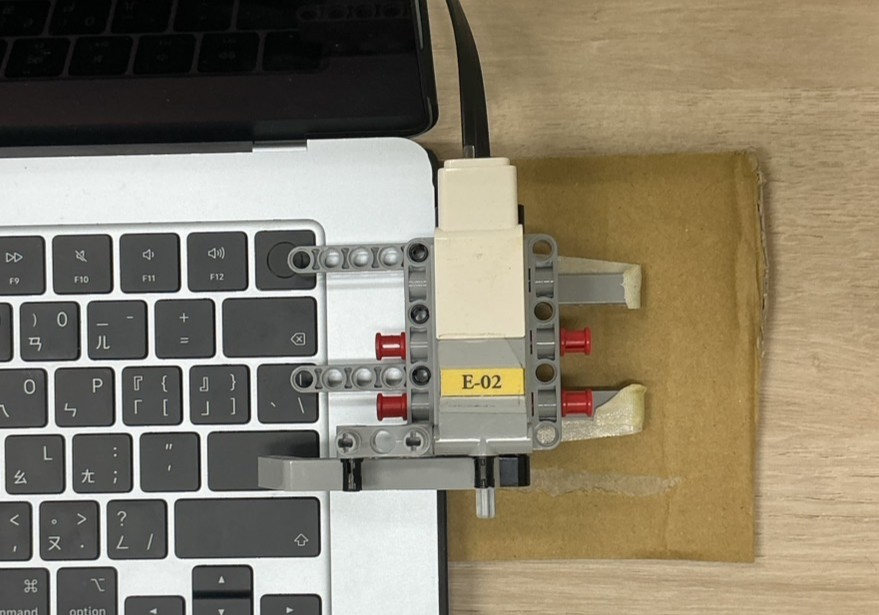
\includegraphics[width=3cm, align=c]{image/數據同步器.JPG} 
         \tabularnewline 
        \hline

        \centering 名稱 & \centering 暗室 &  &   \tabularnewline 
        \hline
        \centering 圖片 & 
        \centering 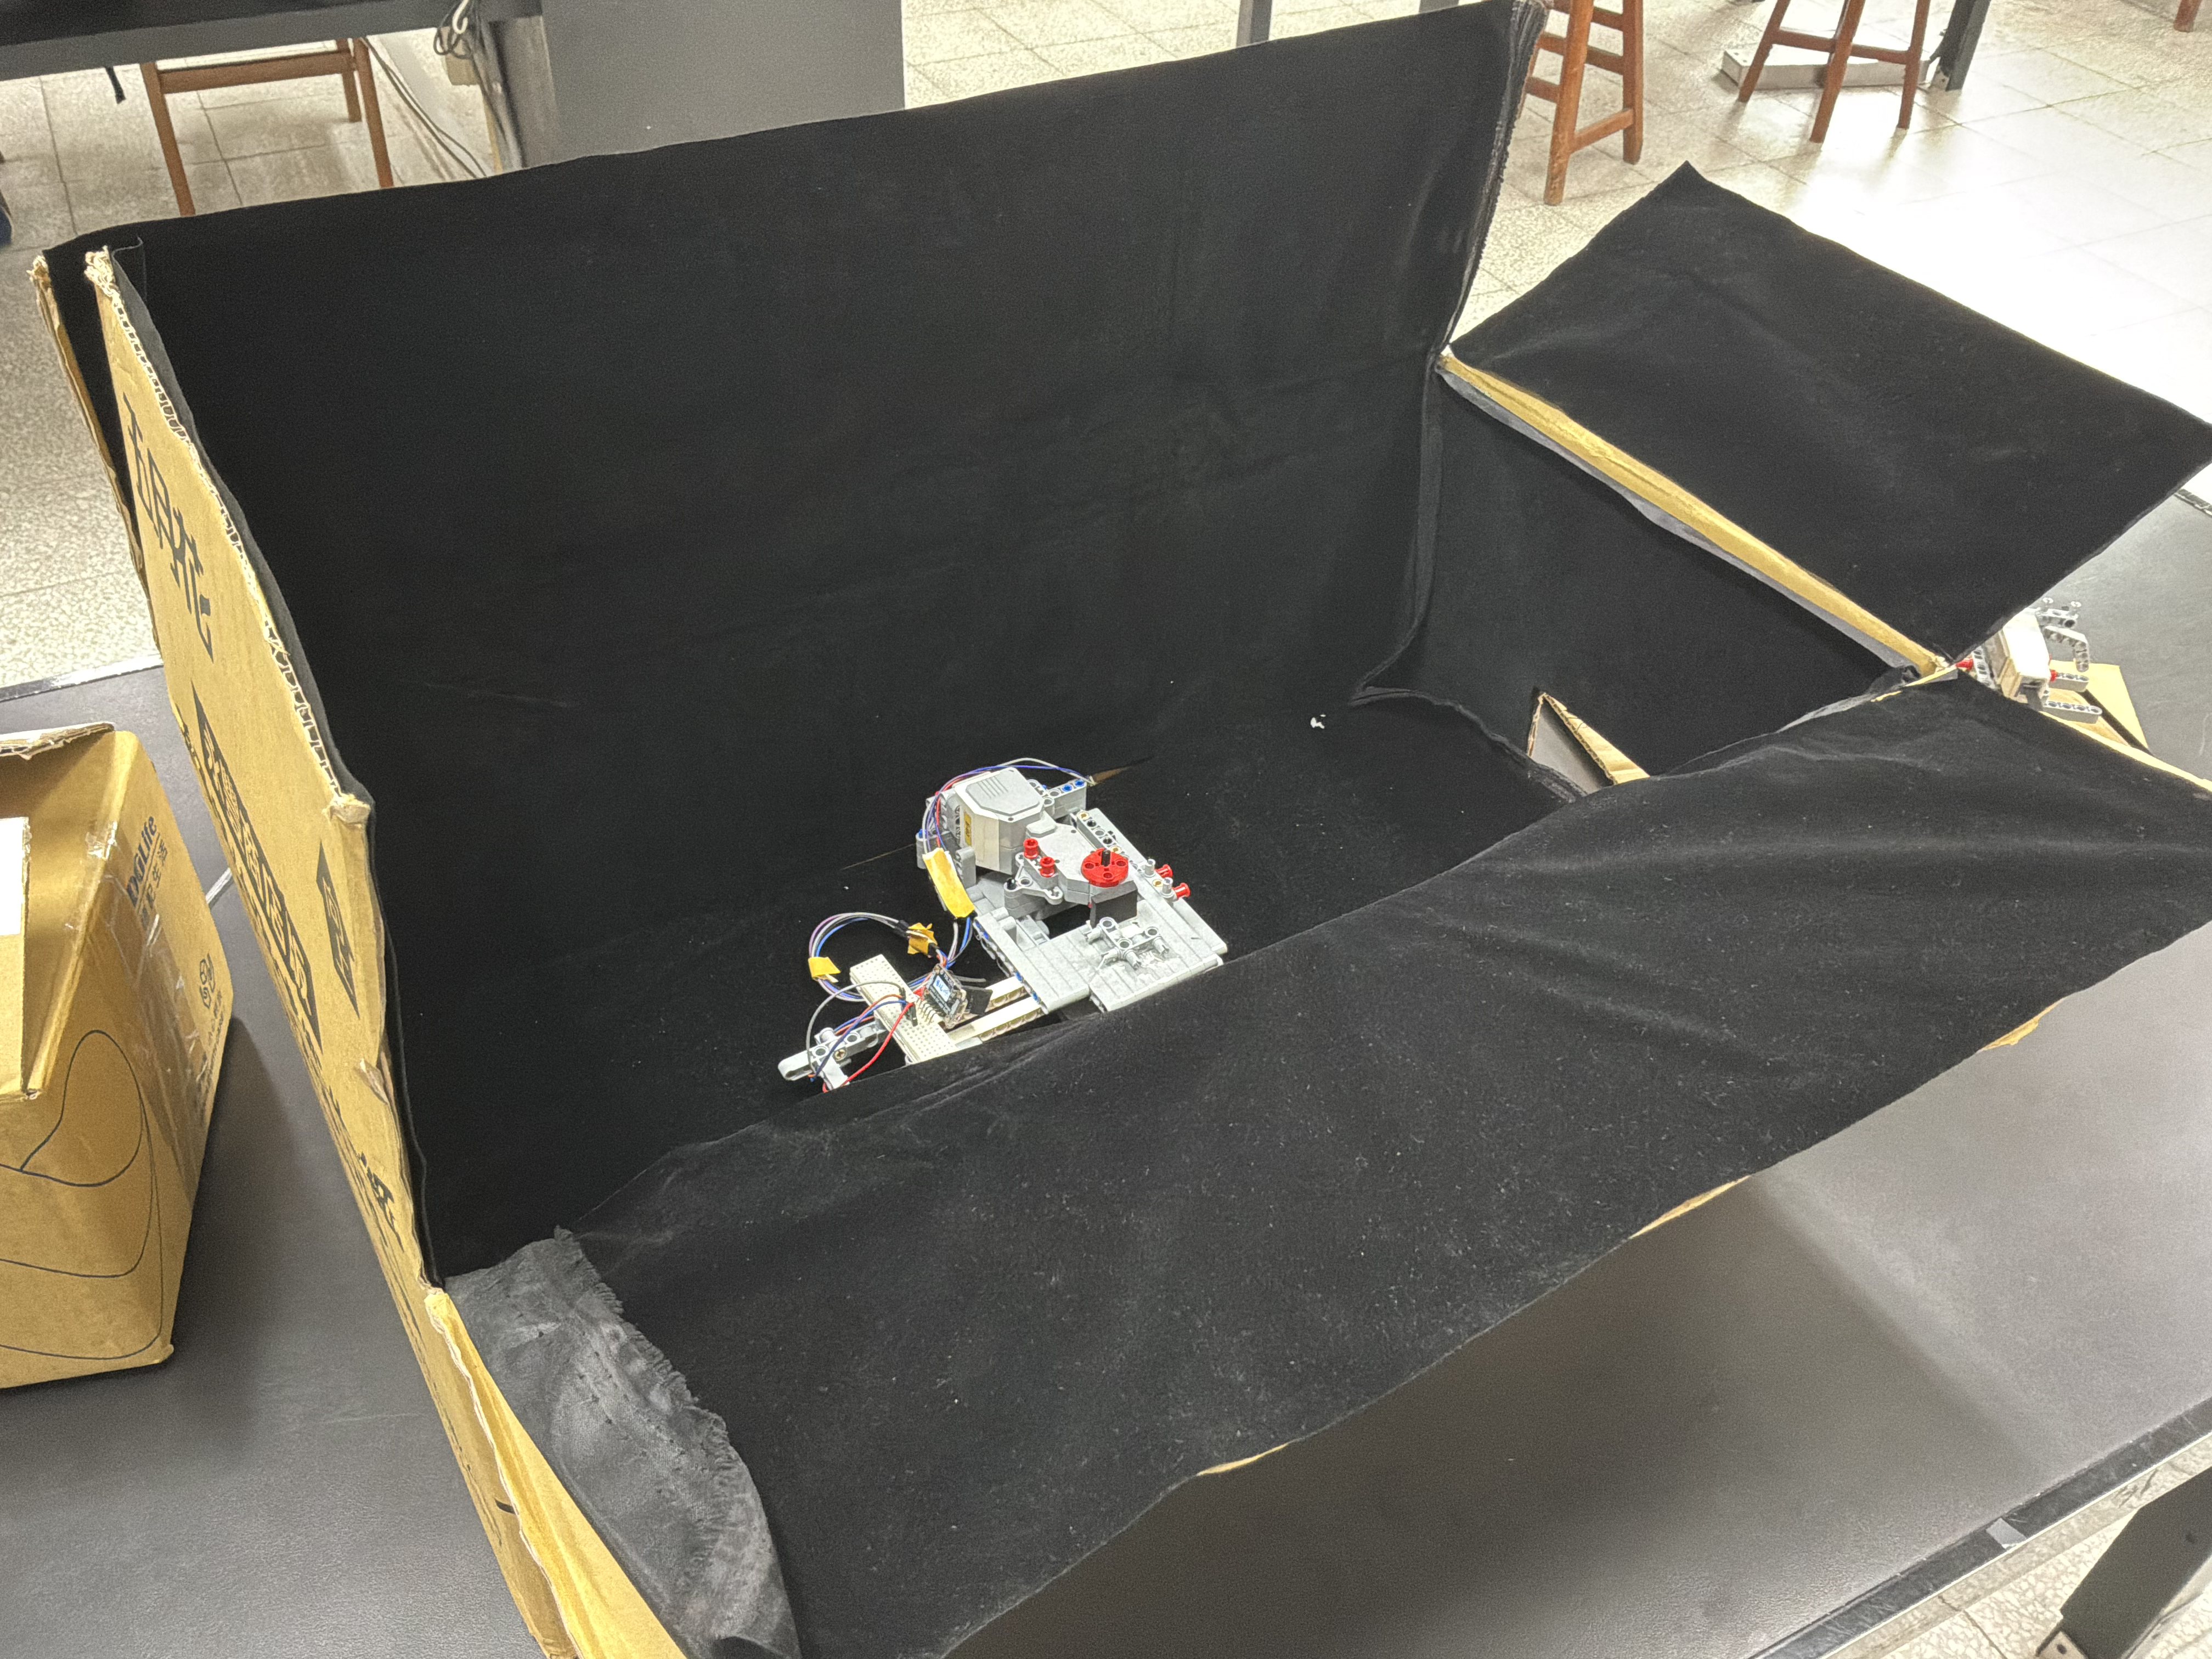
\includegraphics[width=3cm, align=c]{image/暗室.png} &  &
         \tabularnewline 
        \hline
    \end{tabular}
\end{table}
\subsubsection*{說明}
\begin{itemize}
    \item 氦氖雷射（He-Ne laser）：波長 $632.8\,\mathrm{nm}$、功率 $5\,\mathrm{mW}$，作為光源。
    \item TSL2591 數位光感測模組（Adafruit）：收光面積 $0.28\,\mathrm{mm}^2$，使用全光譜 CH0 與紅外線 CH1，並以 CH0 減 CH1 作為散射強度。
    \item Arduino Uno 微控制器：讀取感測器並將資料傳至電腦。
    \item 旋轉臂：以 LEGO Education MINDSTORMS EV3 零件組裝並由 EV3 馬達驅動，實測半徑 $110\,\mathrm{mm}$；感測器裝於臂端，每 $1^\circ$ 停留量測，臂角範圍為 $0^\circ$ 至 $140^\circ$。
    \item EV3 馬達模組：轉動旋轉臂
    \item 自動數據同步器：同步 ev3 轉動與紀錄數據的資訊
    \item 暗室 : 隔絕實驗室環境光
\end{itemize}

\subsection*{二、樣品配製器材}
\begin{table}[H]
    \setlength{\extrarowheight}{1pt}
    \centering

    \begin{tabular}{|m{2cm}|m{3cm}|m{3cm}|m{3cm}|m{3cm}|}
        \hline
        \centering 名稱 & \centering 聚苯乙烯微球 TM-P0500、TM-P1002 & 聚苯乙烯微球 TM-P0300、TM-P1003 & \centering 方形比色槽 & \centering 微量儀液劑 \tabularnewline \hline
        \centering 圖片 & 
        \centering 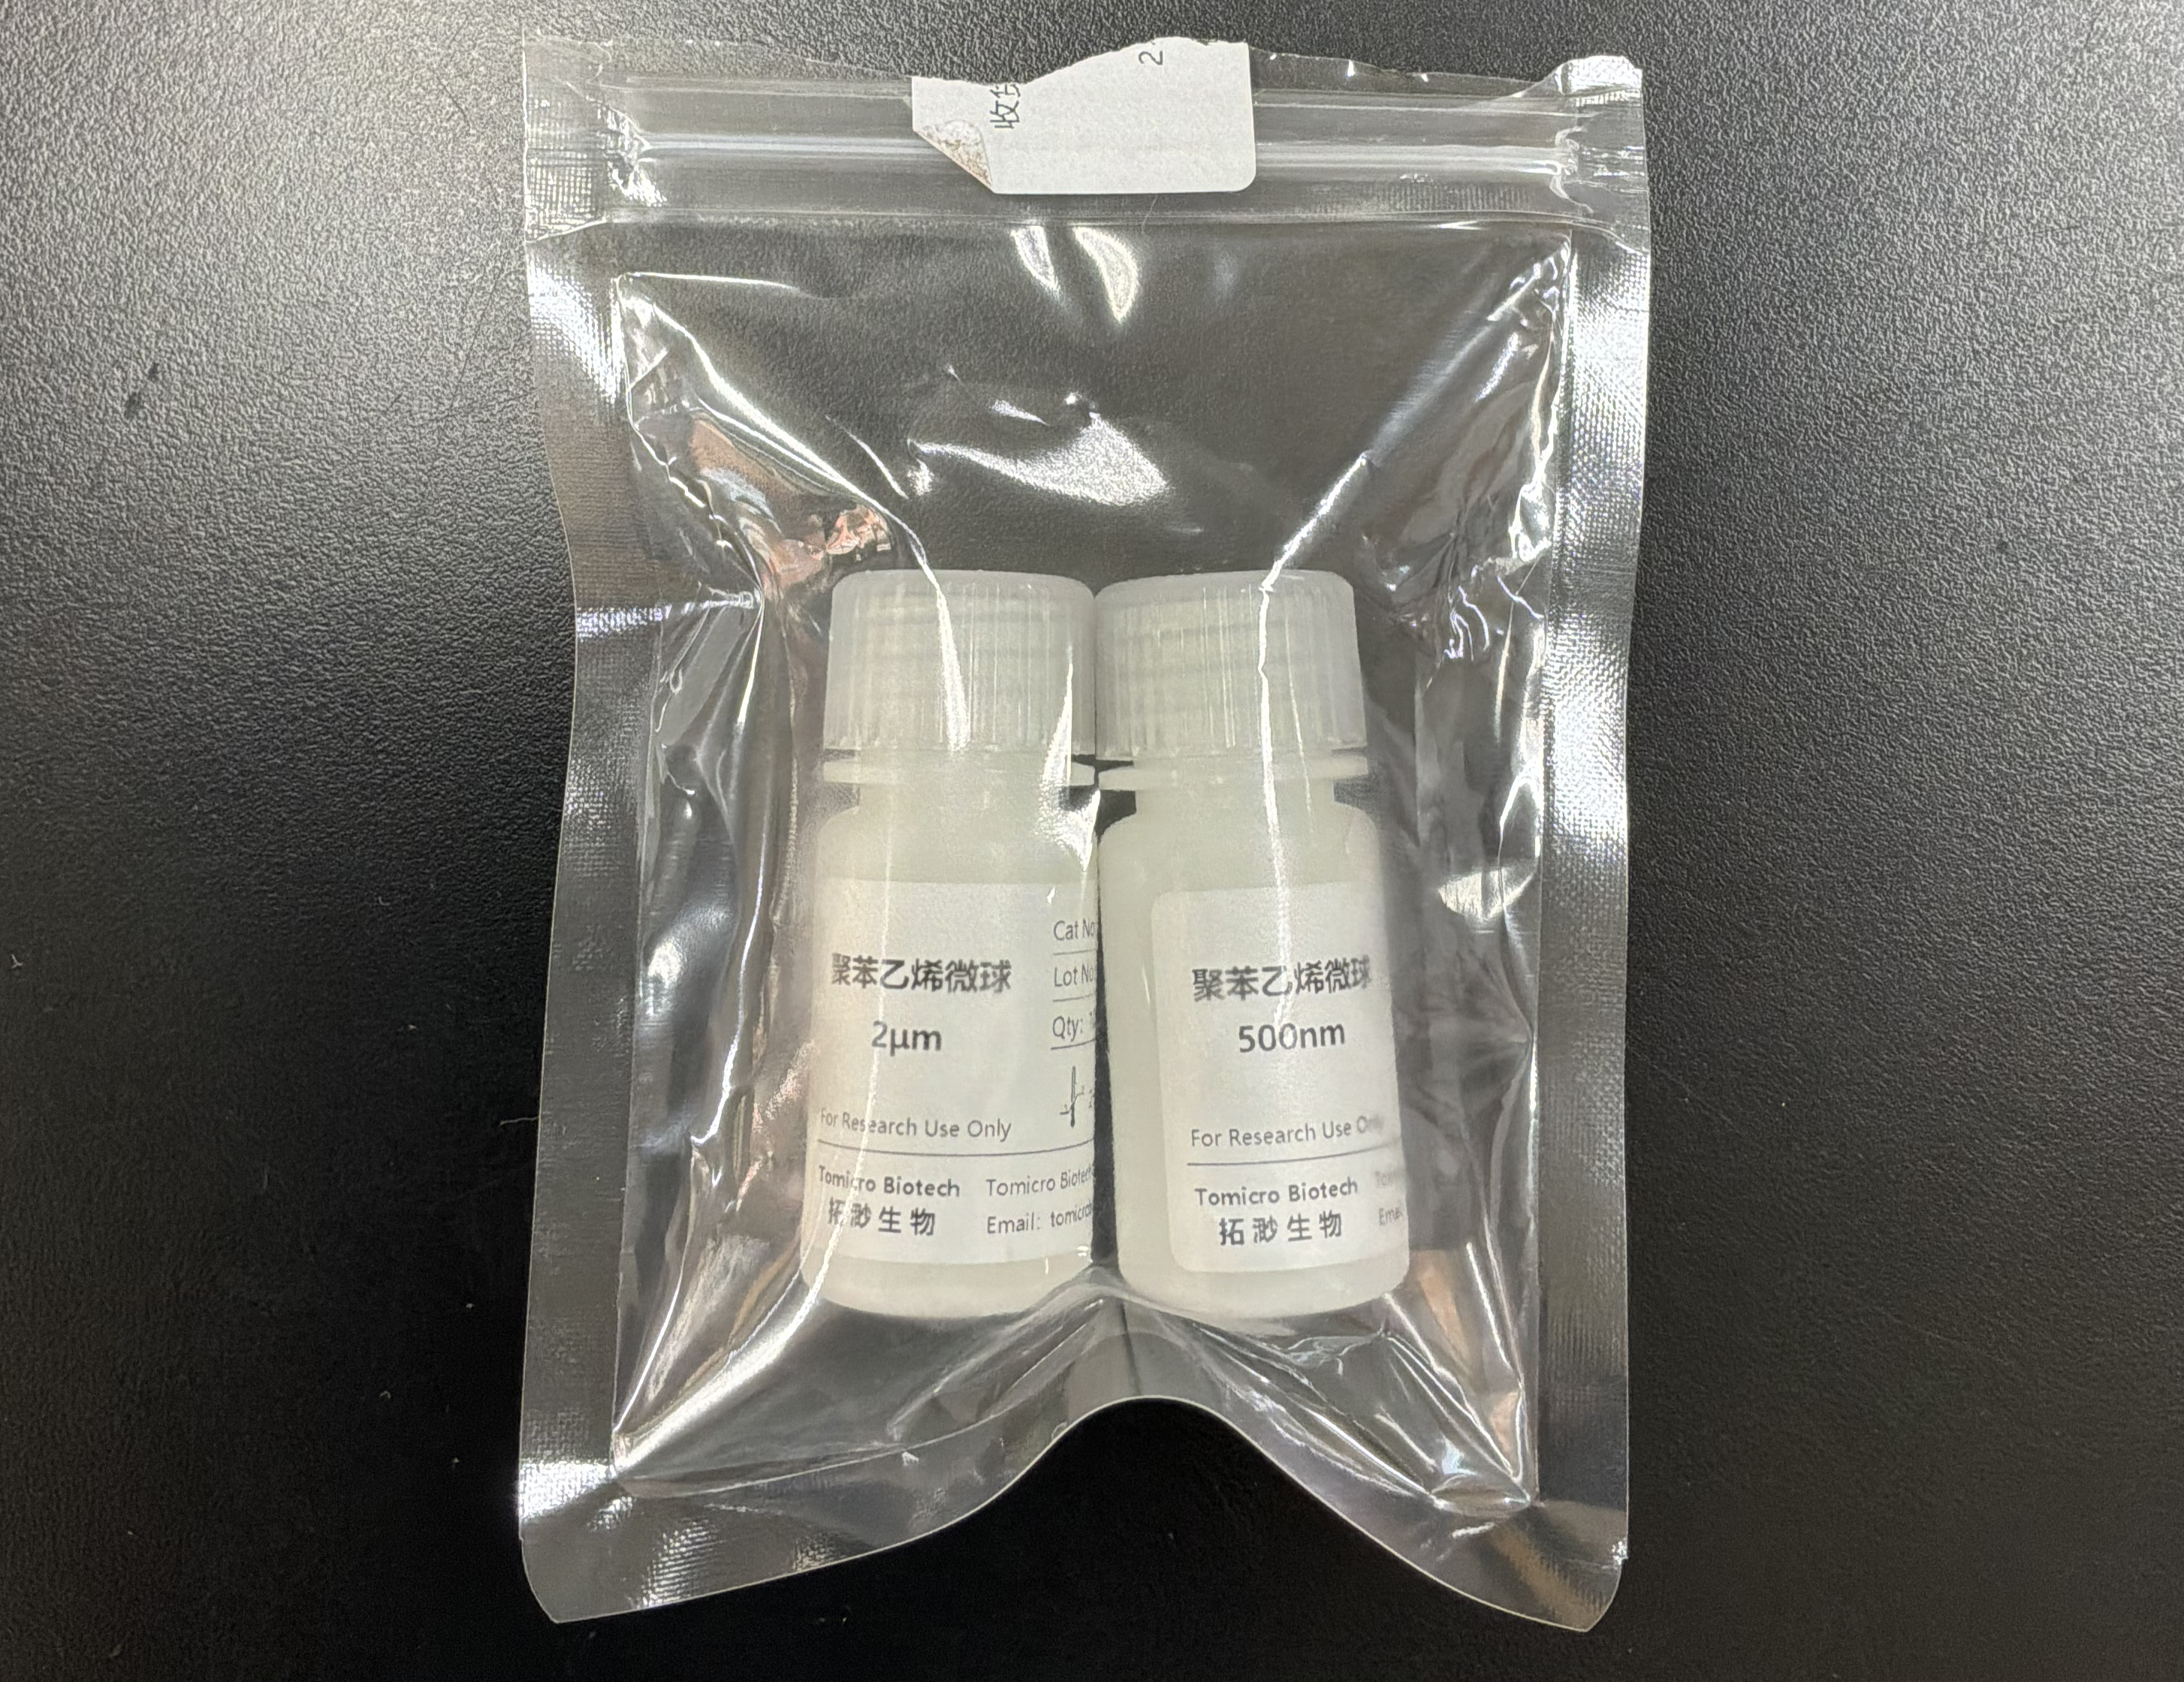
\includegraphics[width=3cm, align=c]{image/微粒 2 500.png} & 
        \centering 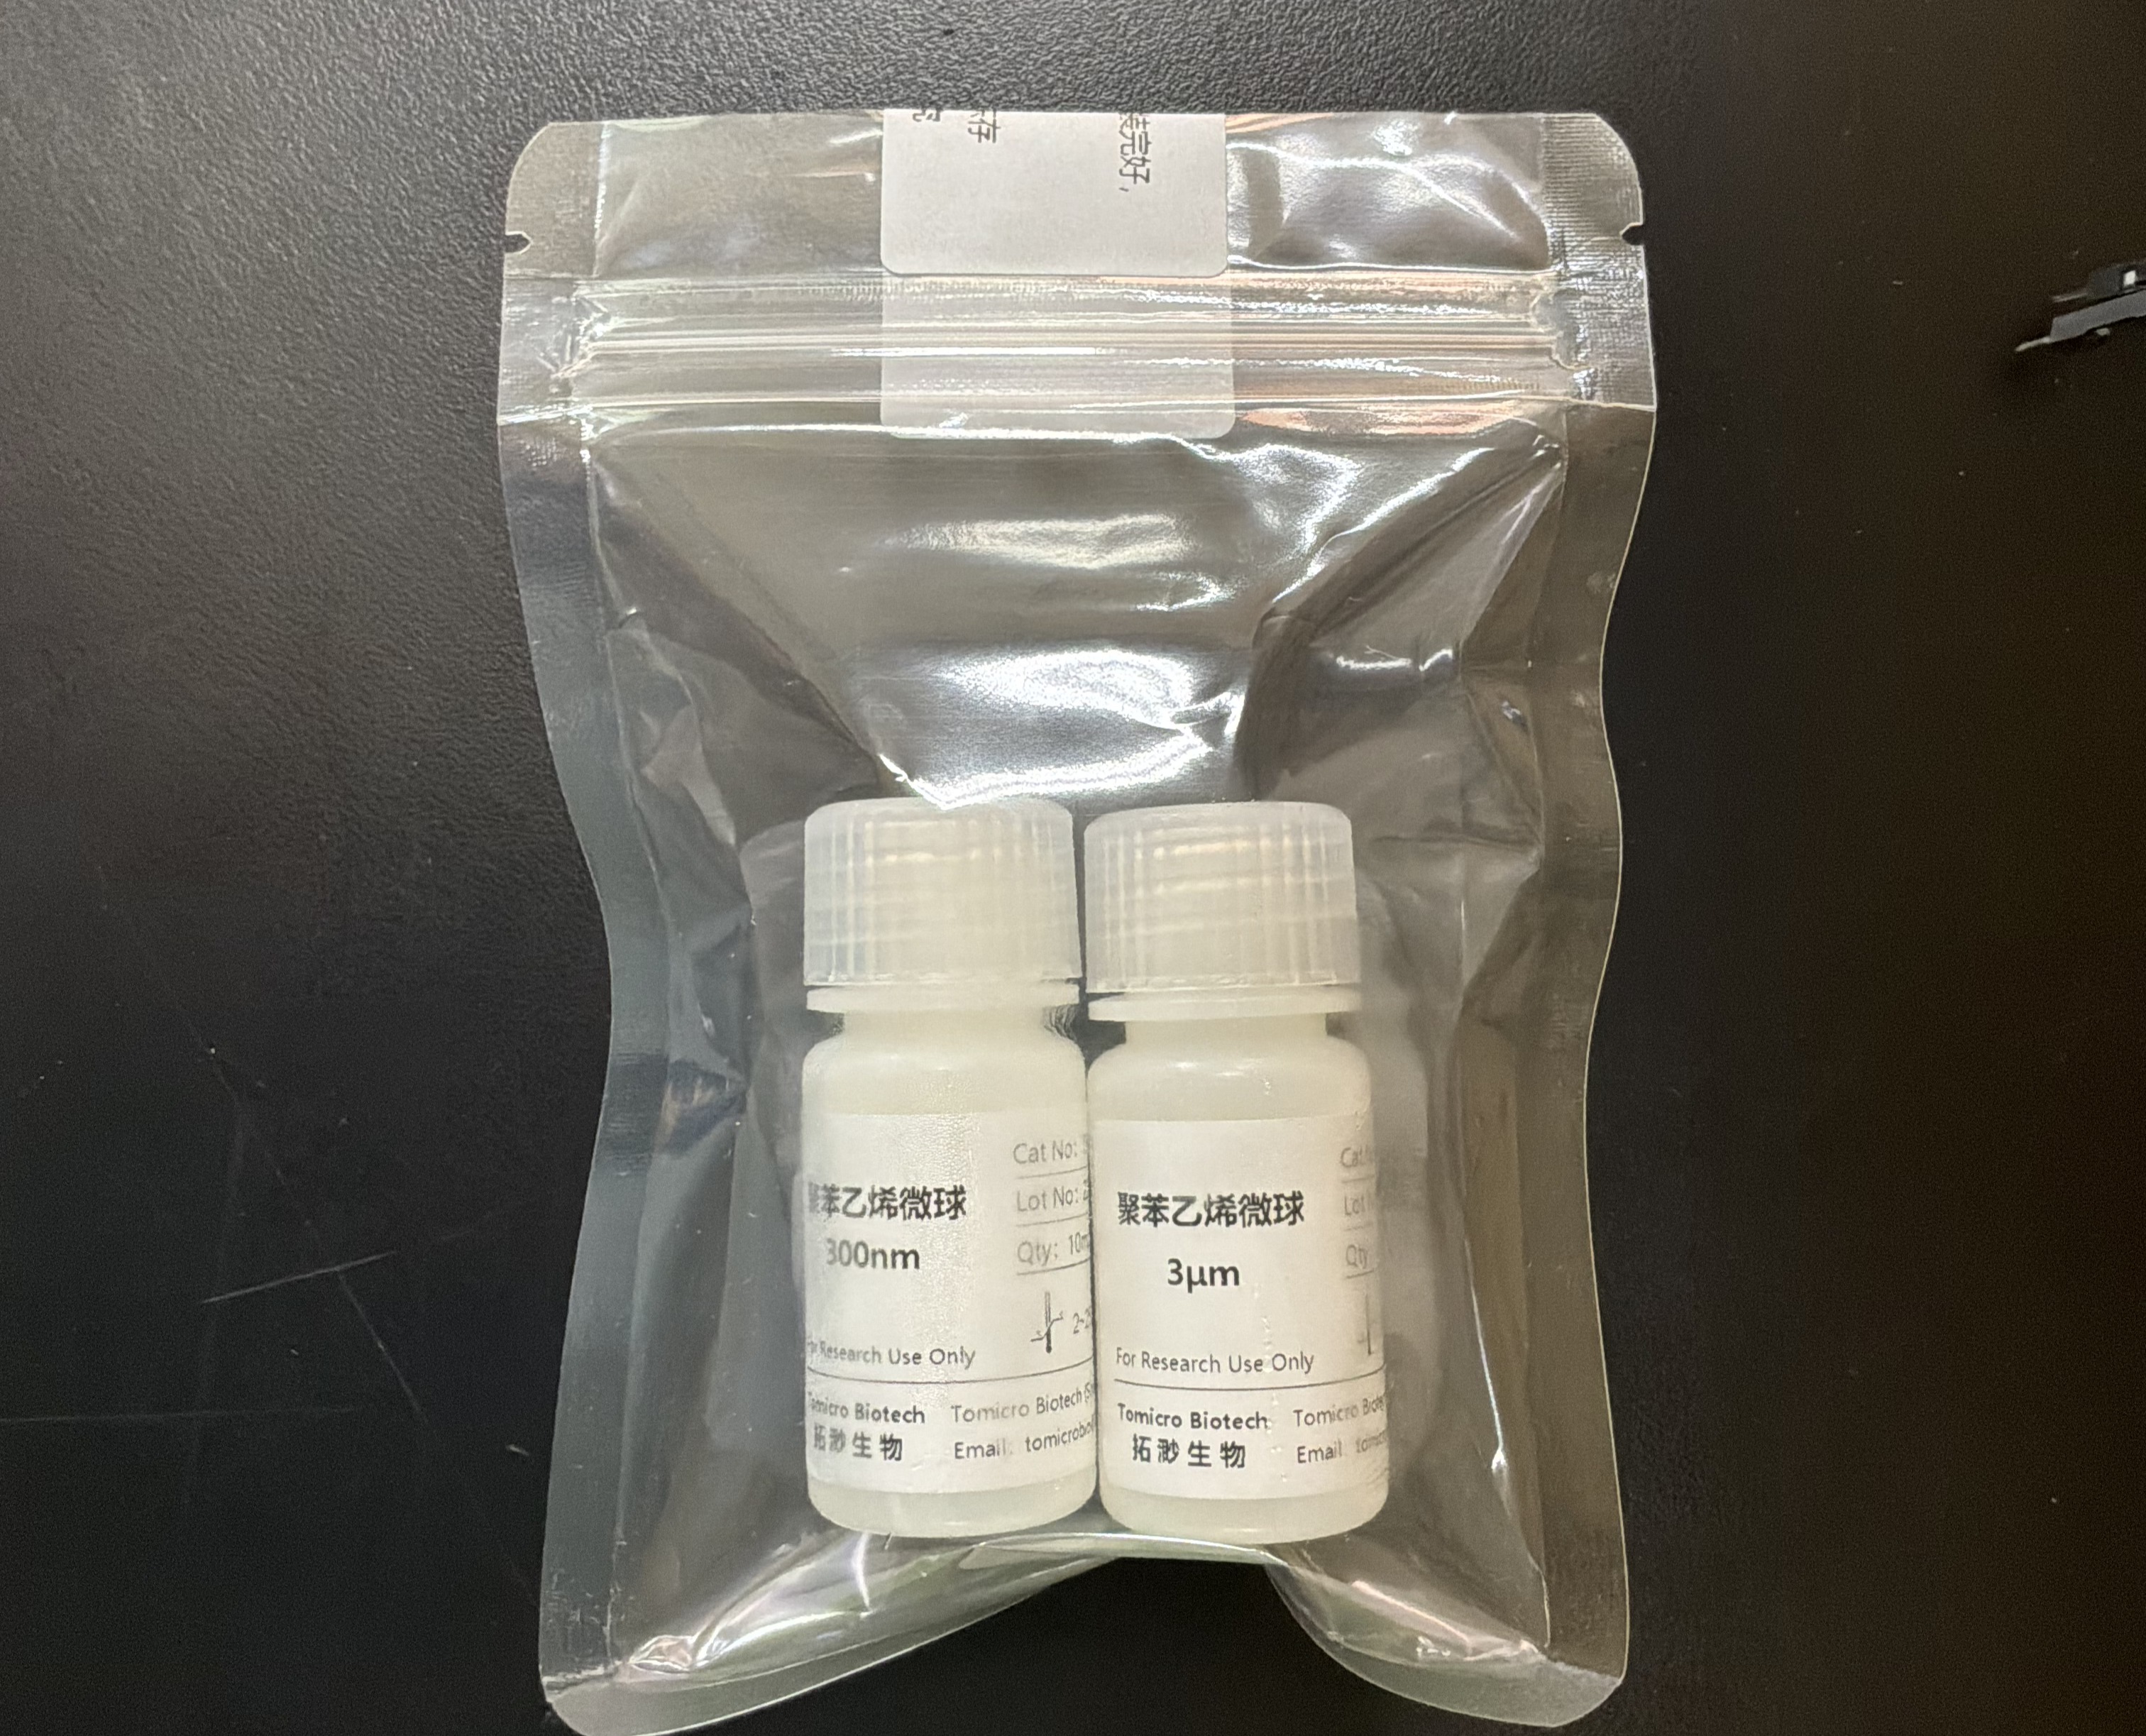
\includegraphics[width=3cm, align=c]{image/微粒 3 300.png} & 
        \centering 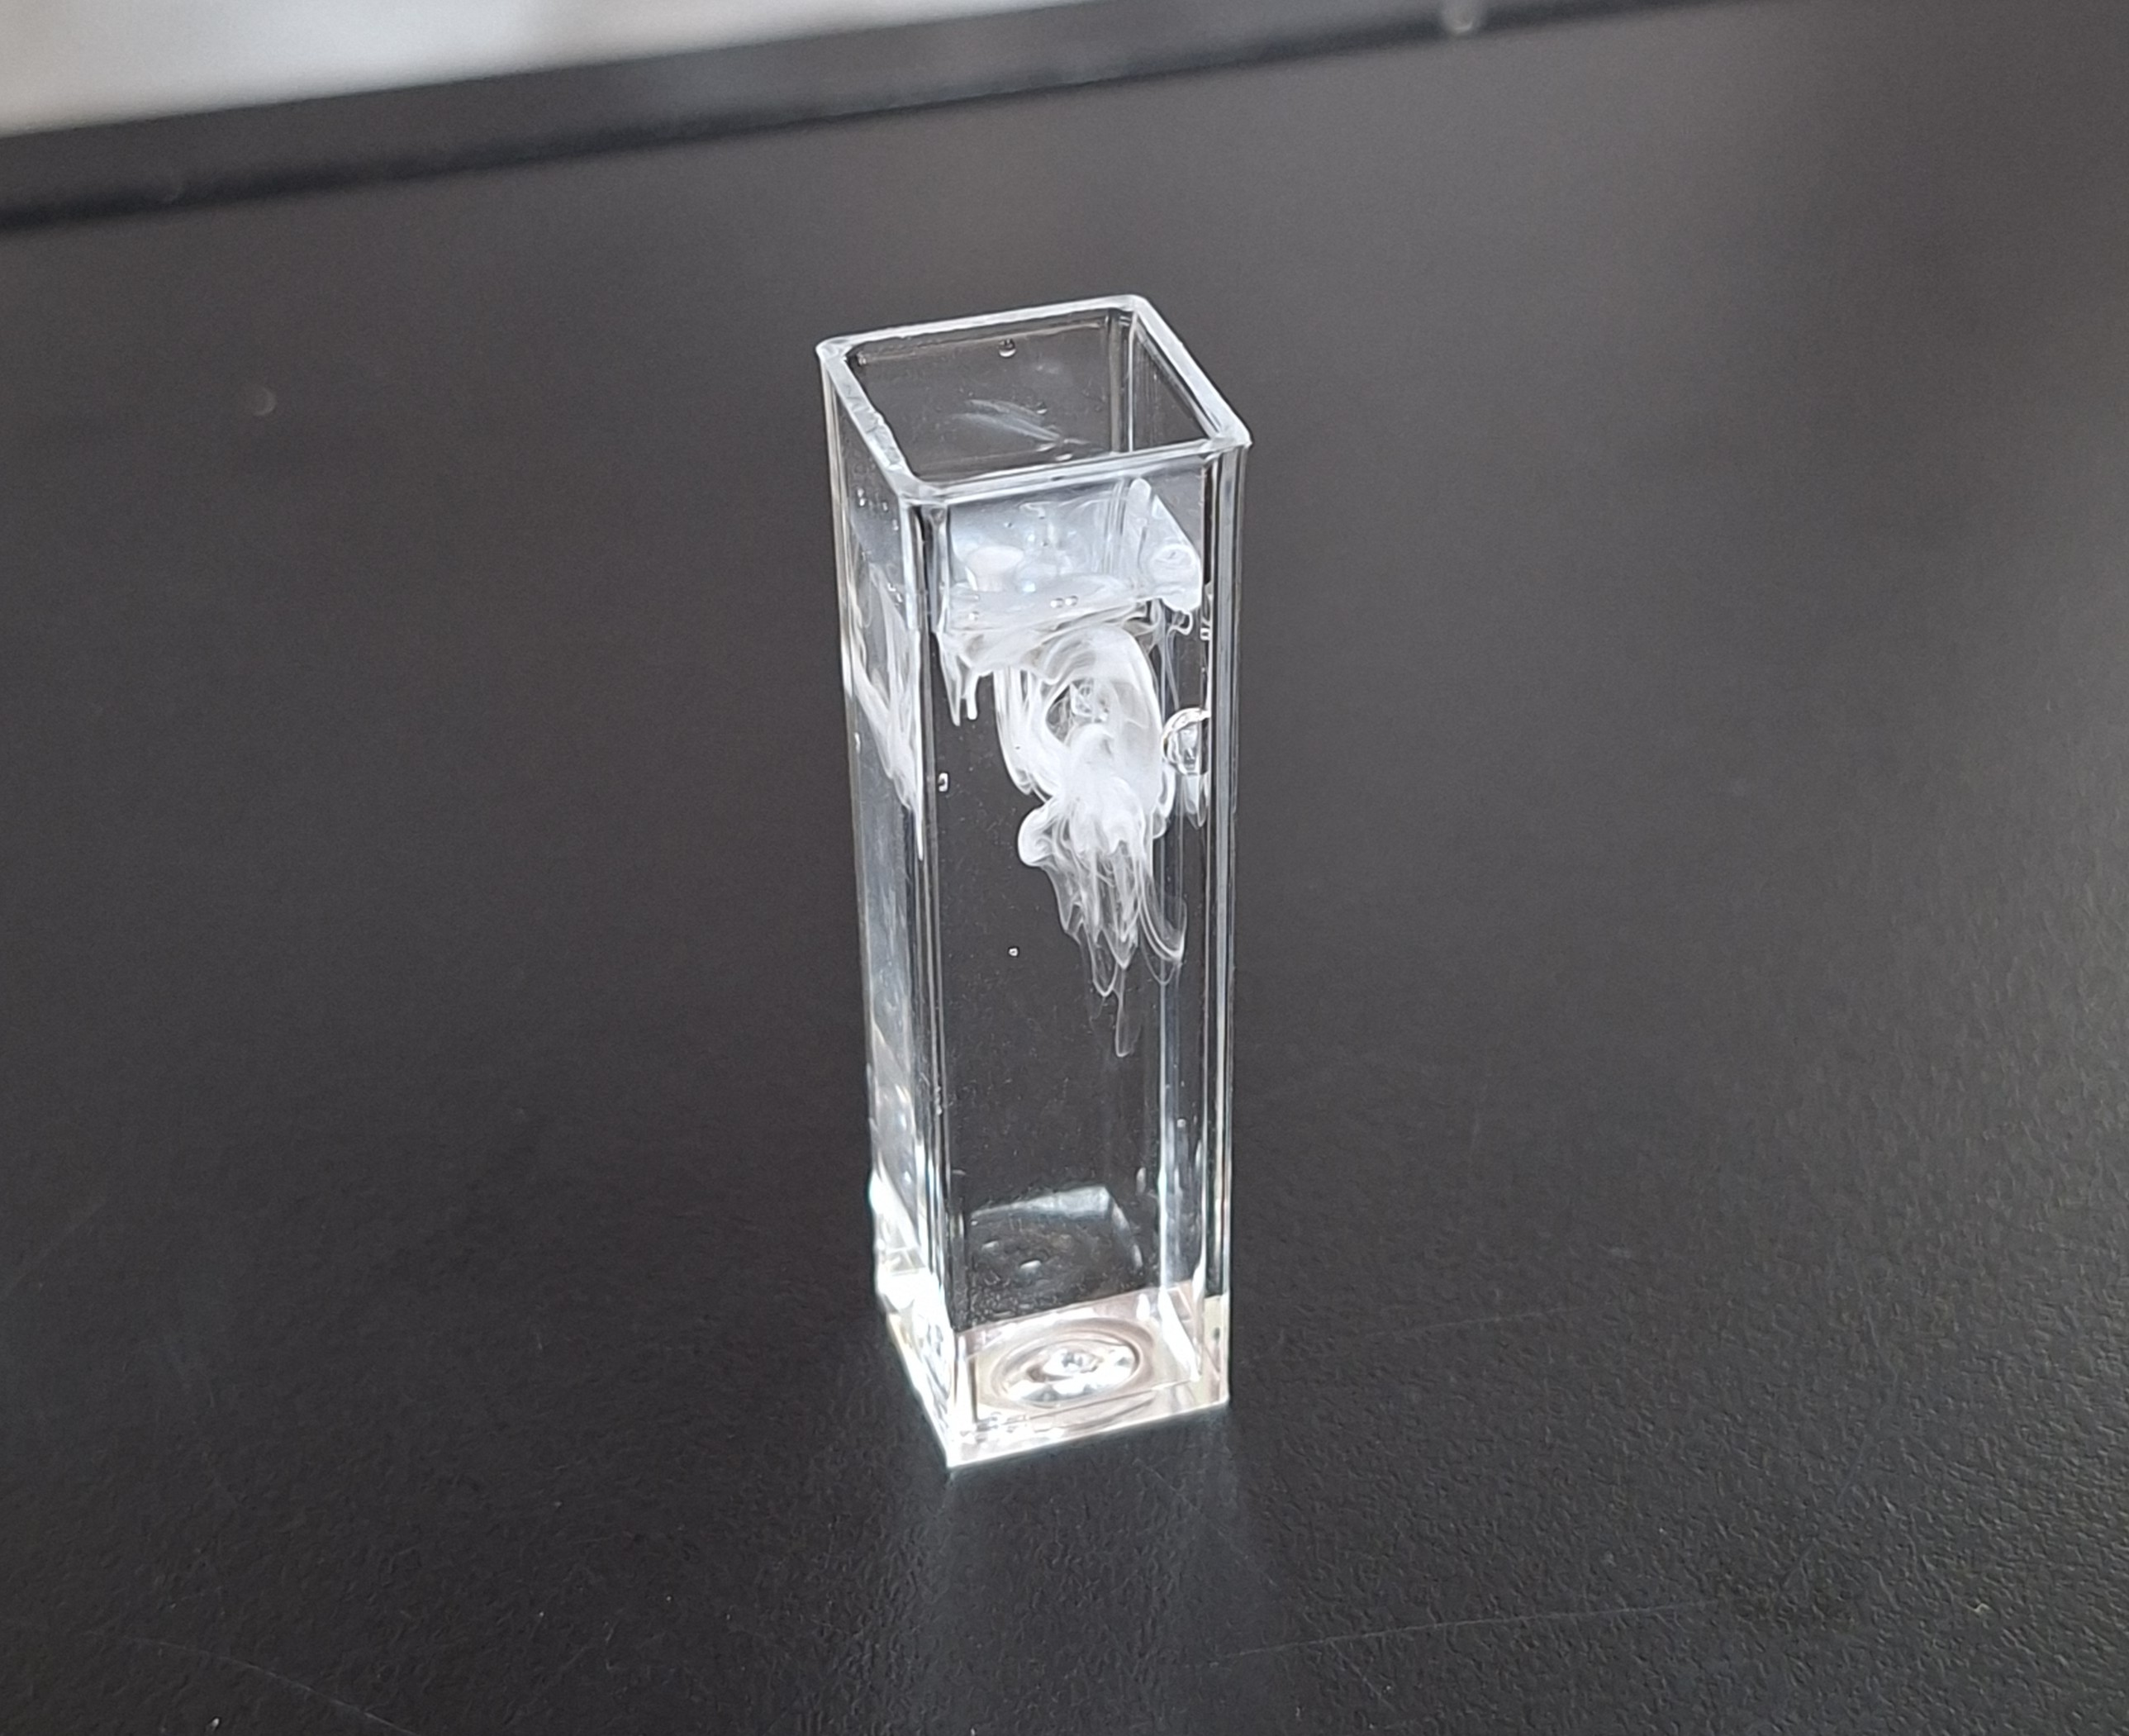
\includegraphics[width=3cm, align=c]{image/方形比色槽.jpg} &
        \centering 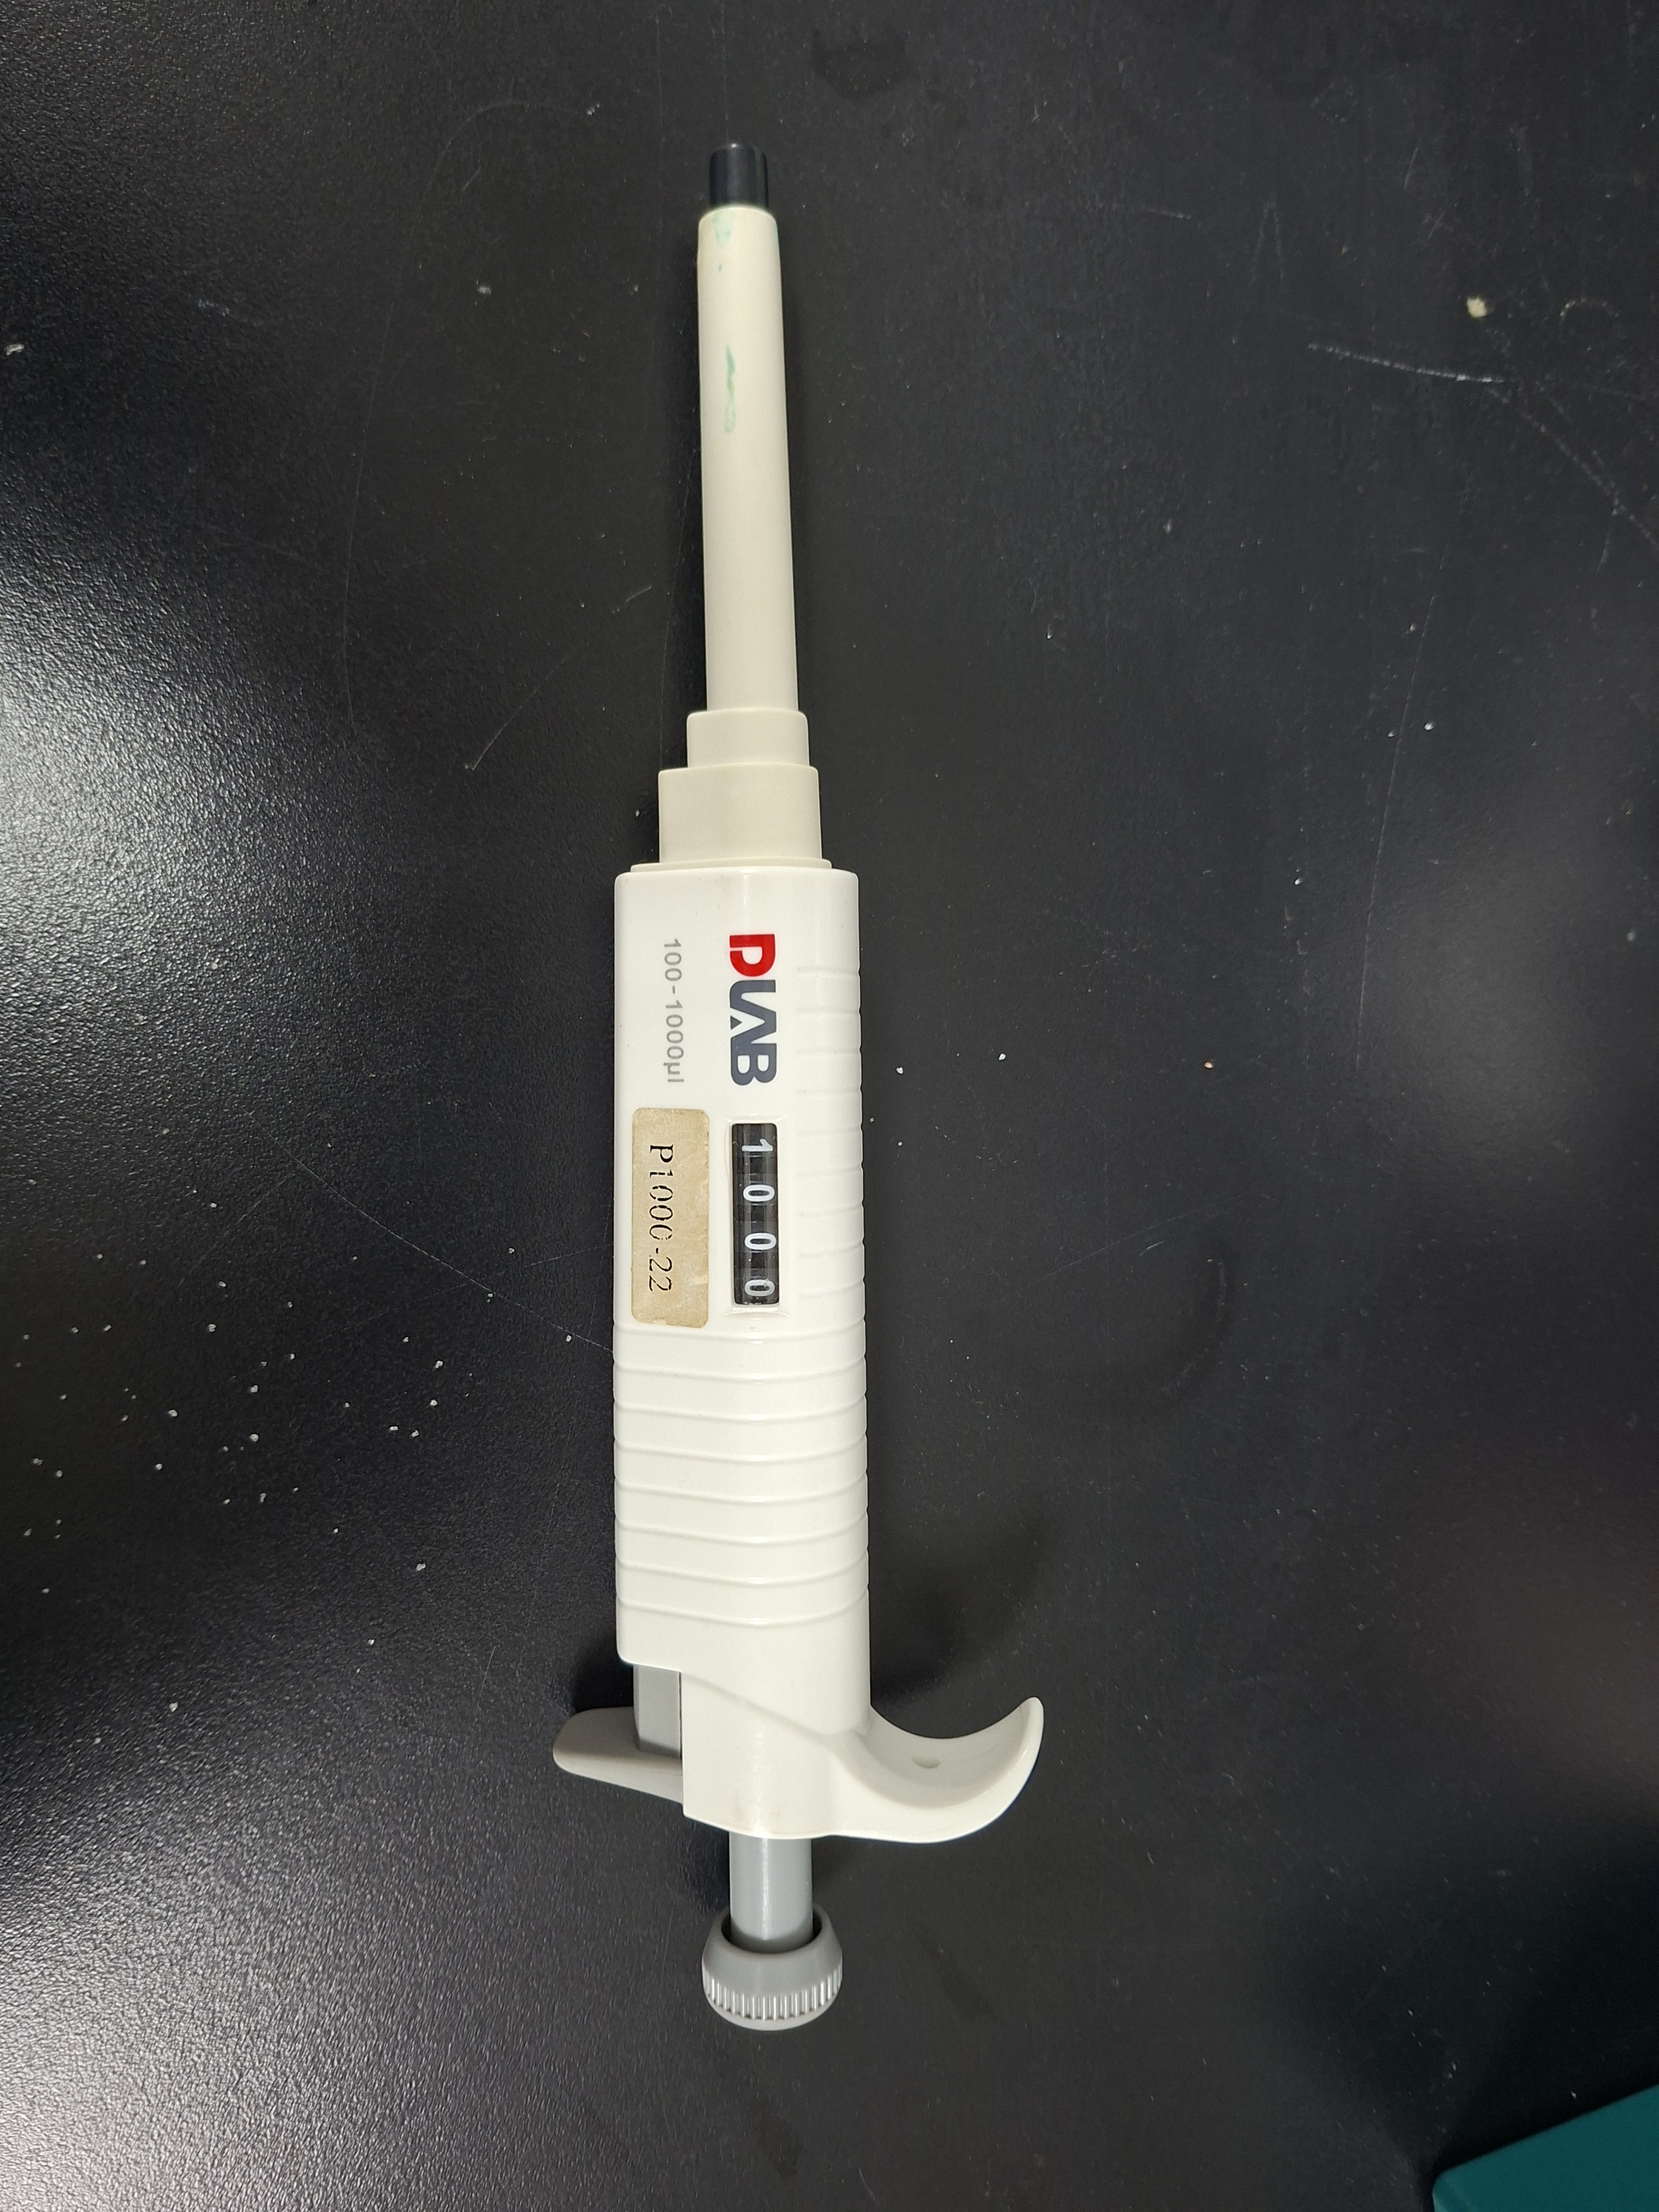
\includegraphics[width=3cm, align=c]{image/微量儀液劑 (100-1000).jpg}  \tabularnewline 
        \hline
    \end{tabular}
\end{table}

\subsubsection*{說明}
\begin{itemize}
    \item 聚苯乙烯微球 TM-P0500（拓渺 Tomicro）：實測粒徑 $492\,\mathrm{nm}$、變異係數（coefficient of variation, CV）$2.1\%$、母液質量濃度 $25\,\mathrm{mg/mL}$。
    \item 聚苯乙烯微球 TM-P1002（拓渺 Tomicro）：實測粒徑 $2.16\,\mu\mathrm{m}$、CV $3.1\%$、母液質量濃度 $25\,\mathrm{mg/mL}$。
    \item Kartell PMMA 方形比色槽：四面透光，光徑 $10\,\mathrm{mm}$，盛裝樣品。
    \item 微量吸管兩支：取母液用吸管最小刻度為 $0.1\,\mu\mathrm{L}$，取水用吸管最小刻度為 $1\,\mu\mathrm{L}$。
    \item 去離子水：作為稀釋用水及空白樣品。
\end{itemize}

\subsection*{三、雷射線偏振角度測量}
\begin{table}[H]
    \setlength{\extrarowheight}{1pt}
    \centering

    \begin{tabular}{|m{2cm}|m{3cm}|m{3cm}|m{3cm}|}
        \hline
        \centering 名稱 & \centering 無偏振雷射筆 & \centering 偏振片 & \centering 支撐架 \tabularnewline \hline
        \centering 圖片 & 
        \centering 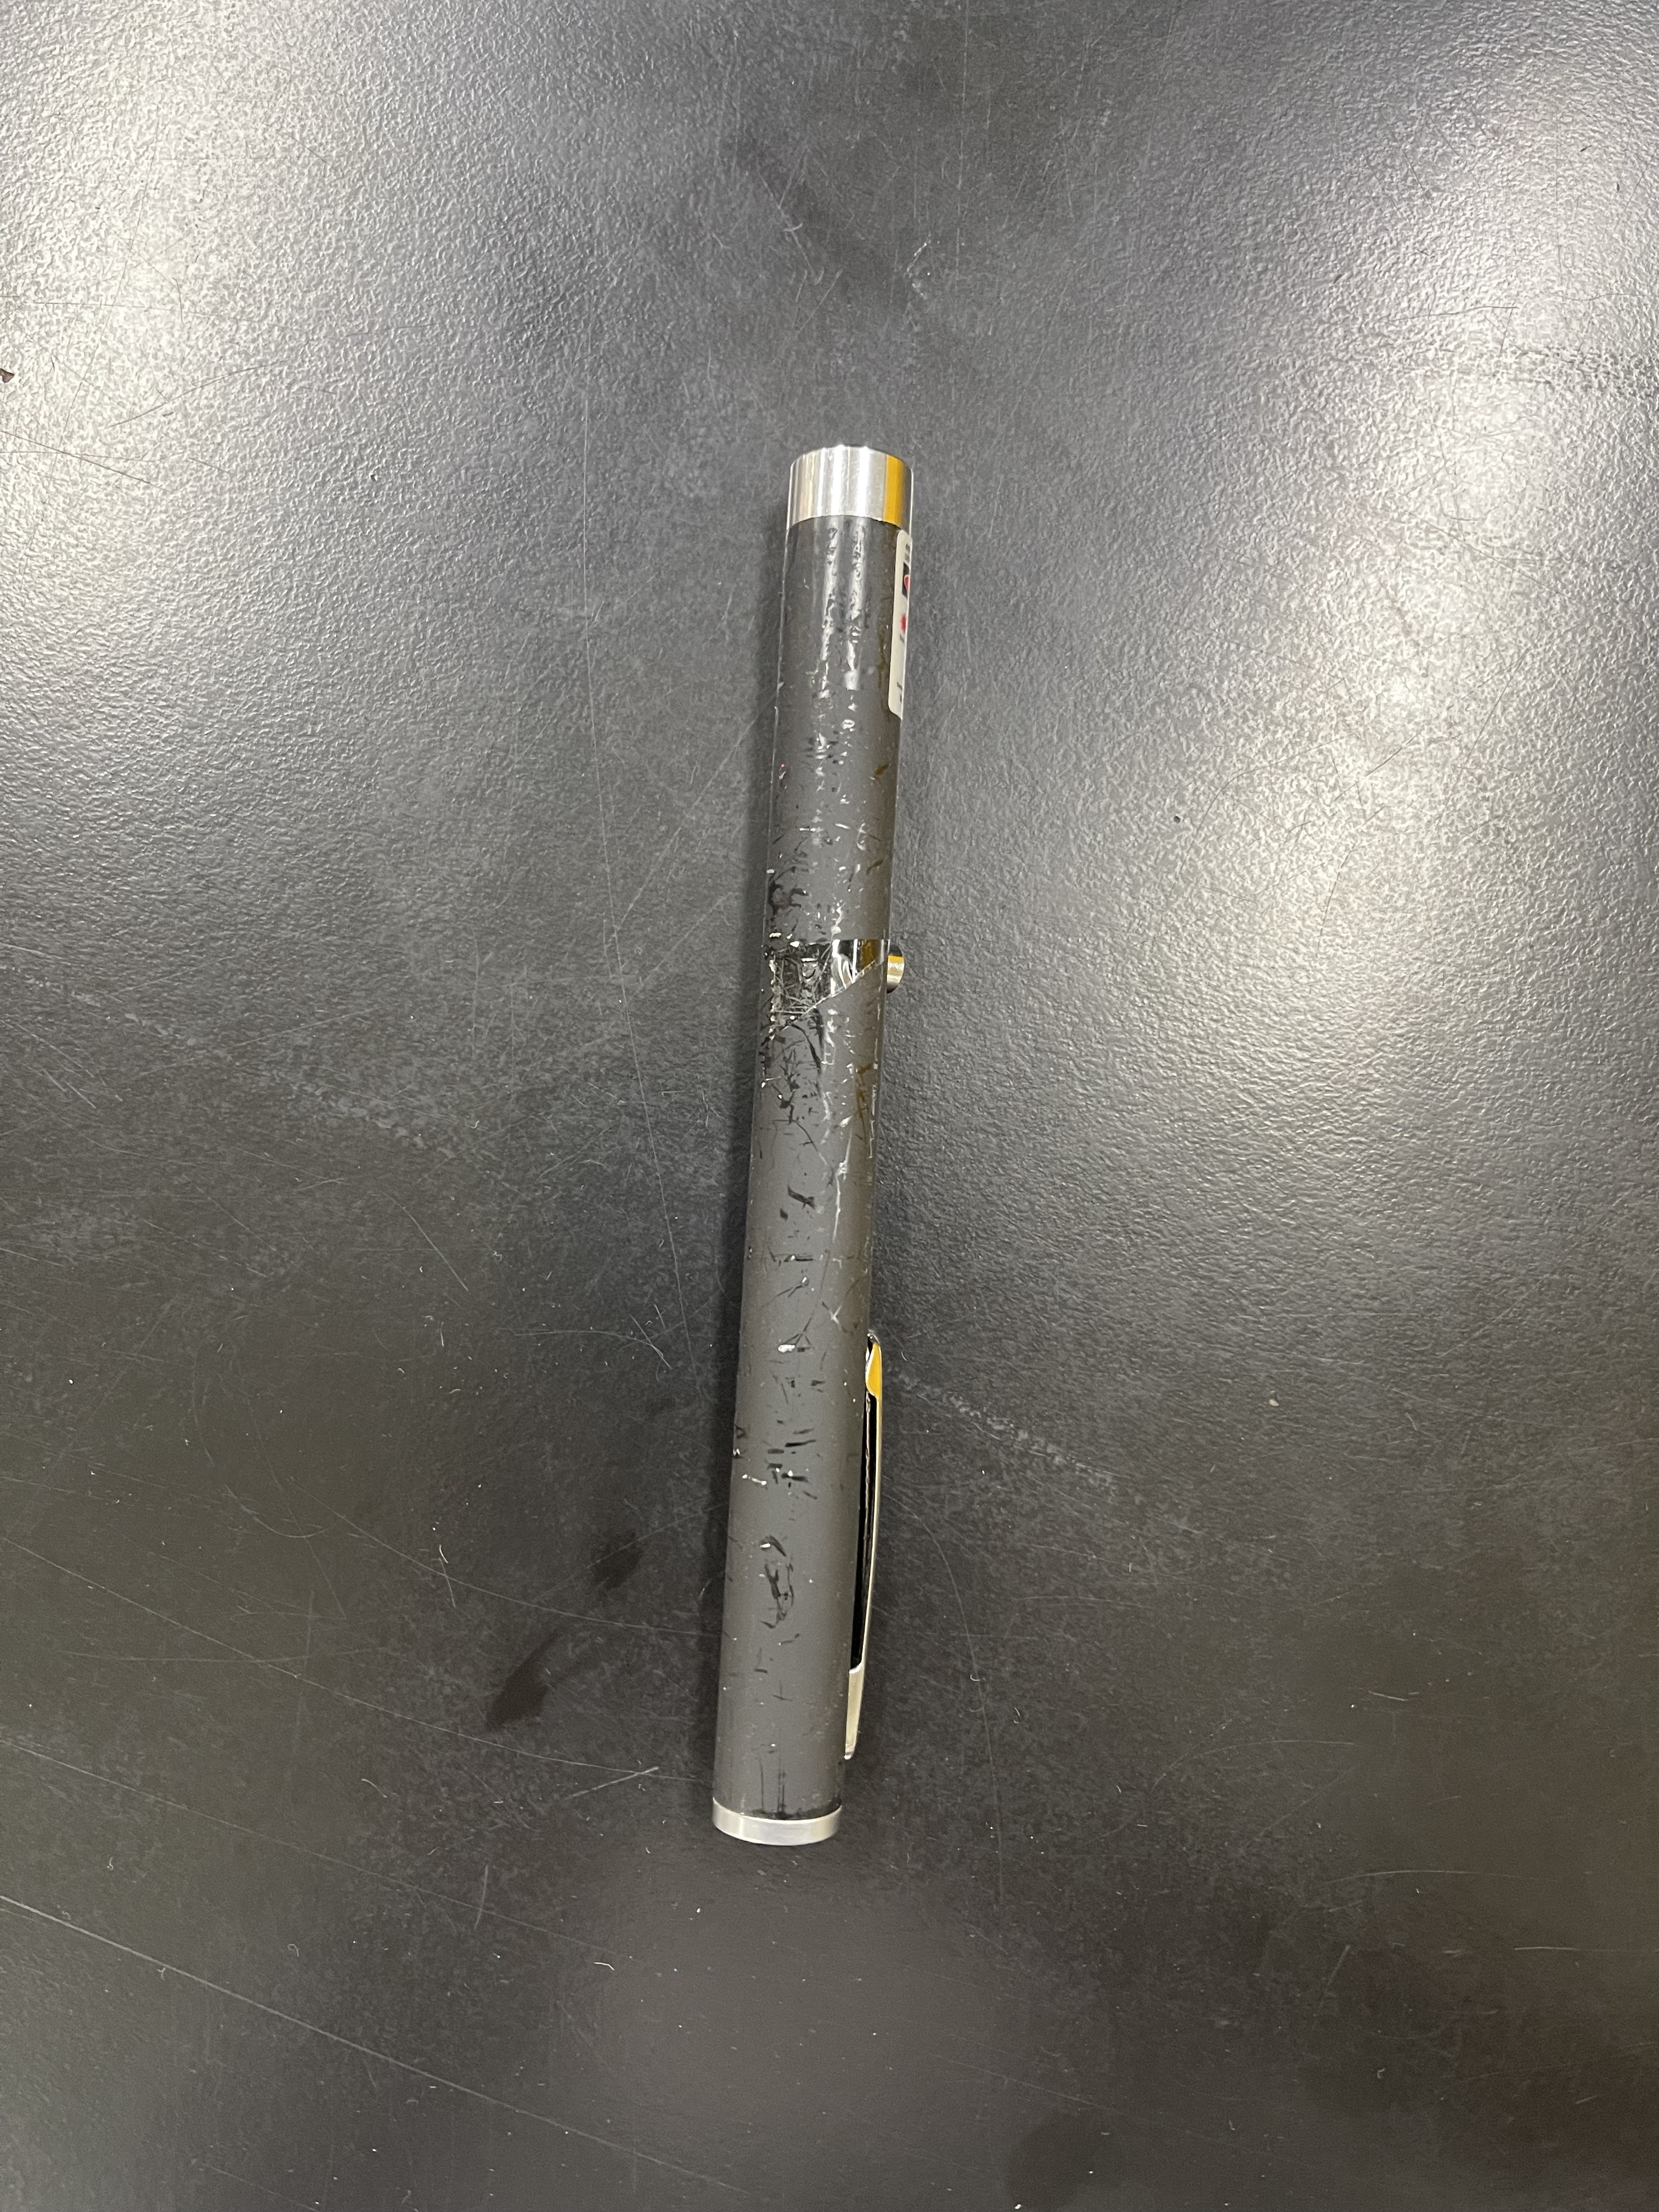
\includegraphics[width=3cm, align=c]{image/雷射筆.jpg} & 
        \centering 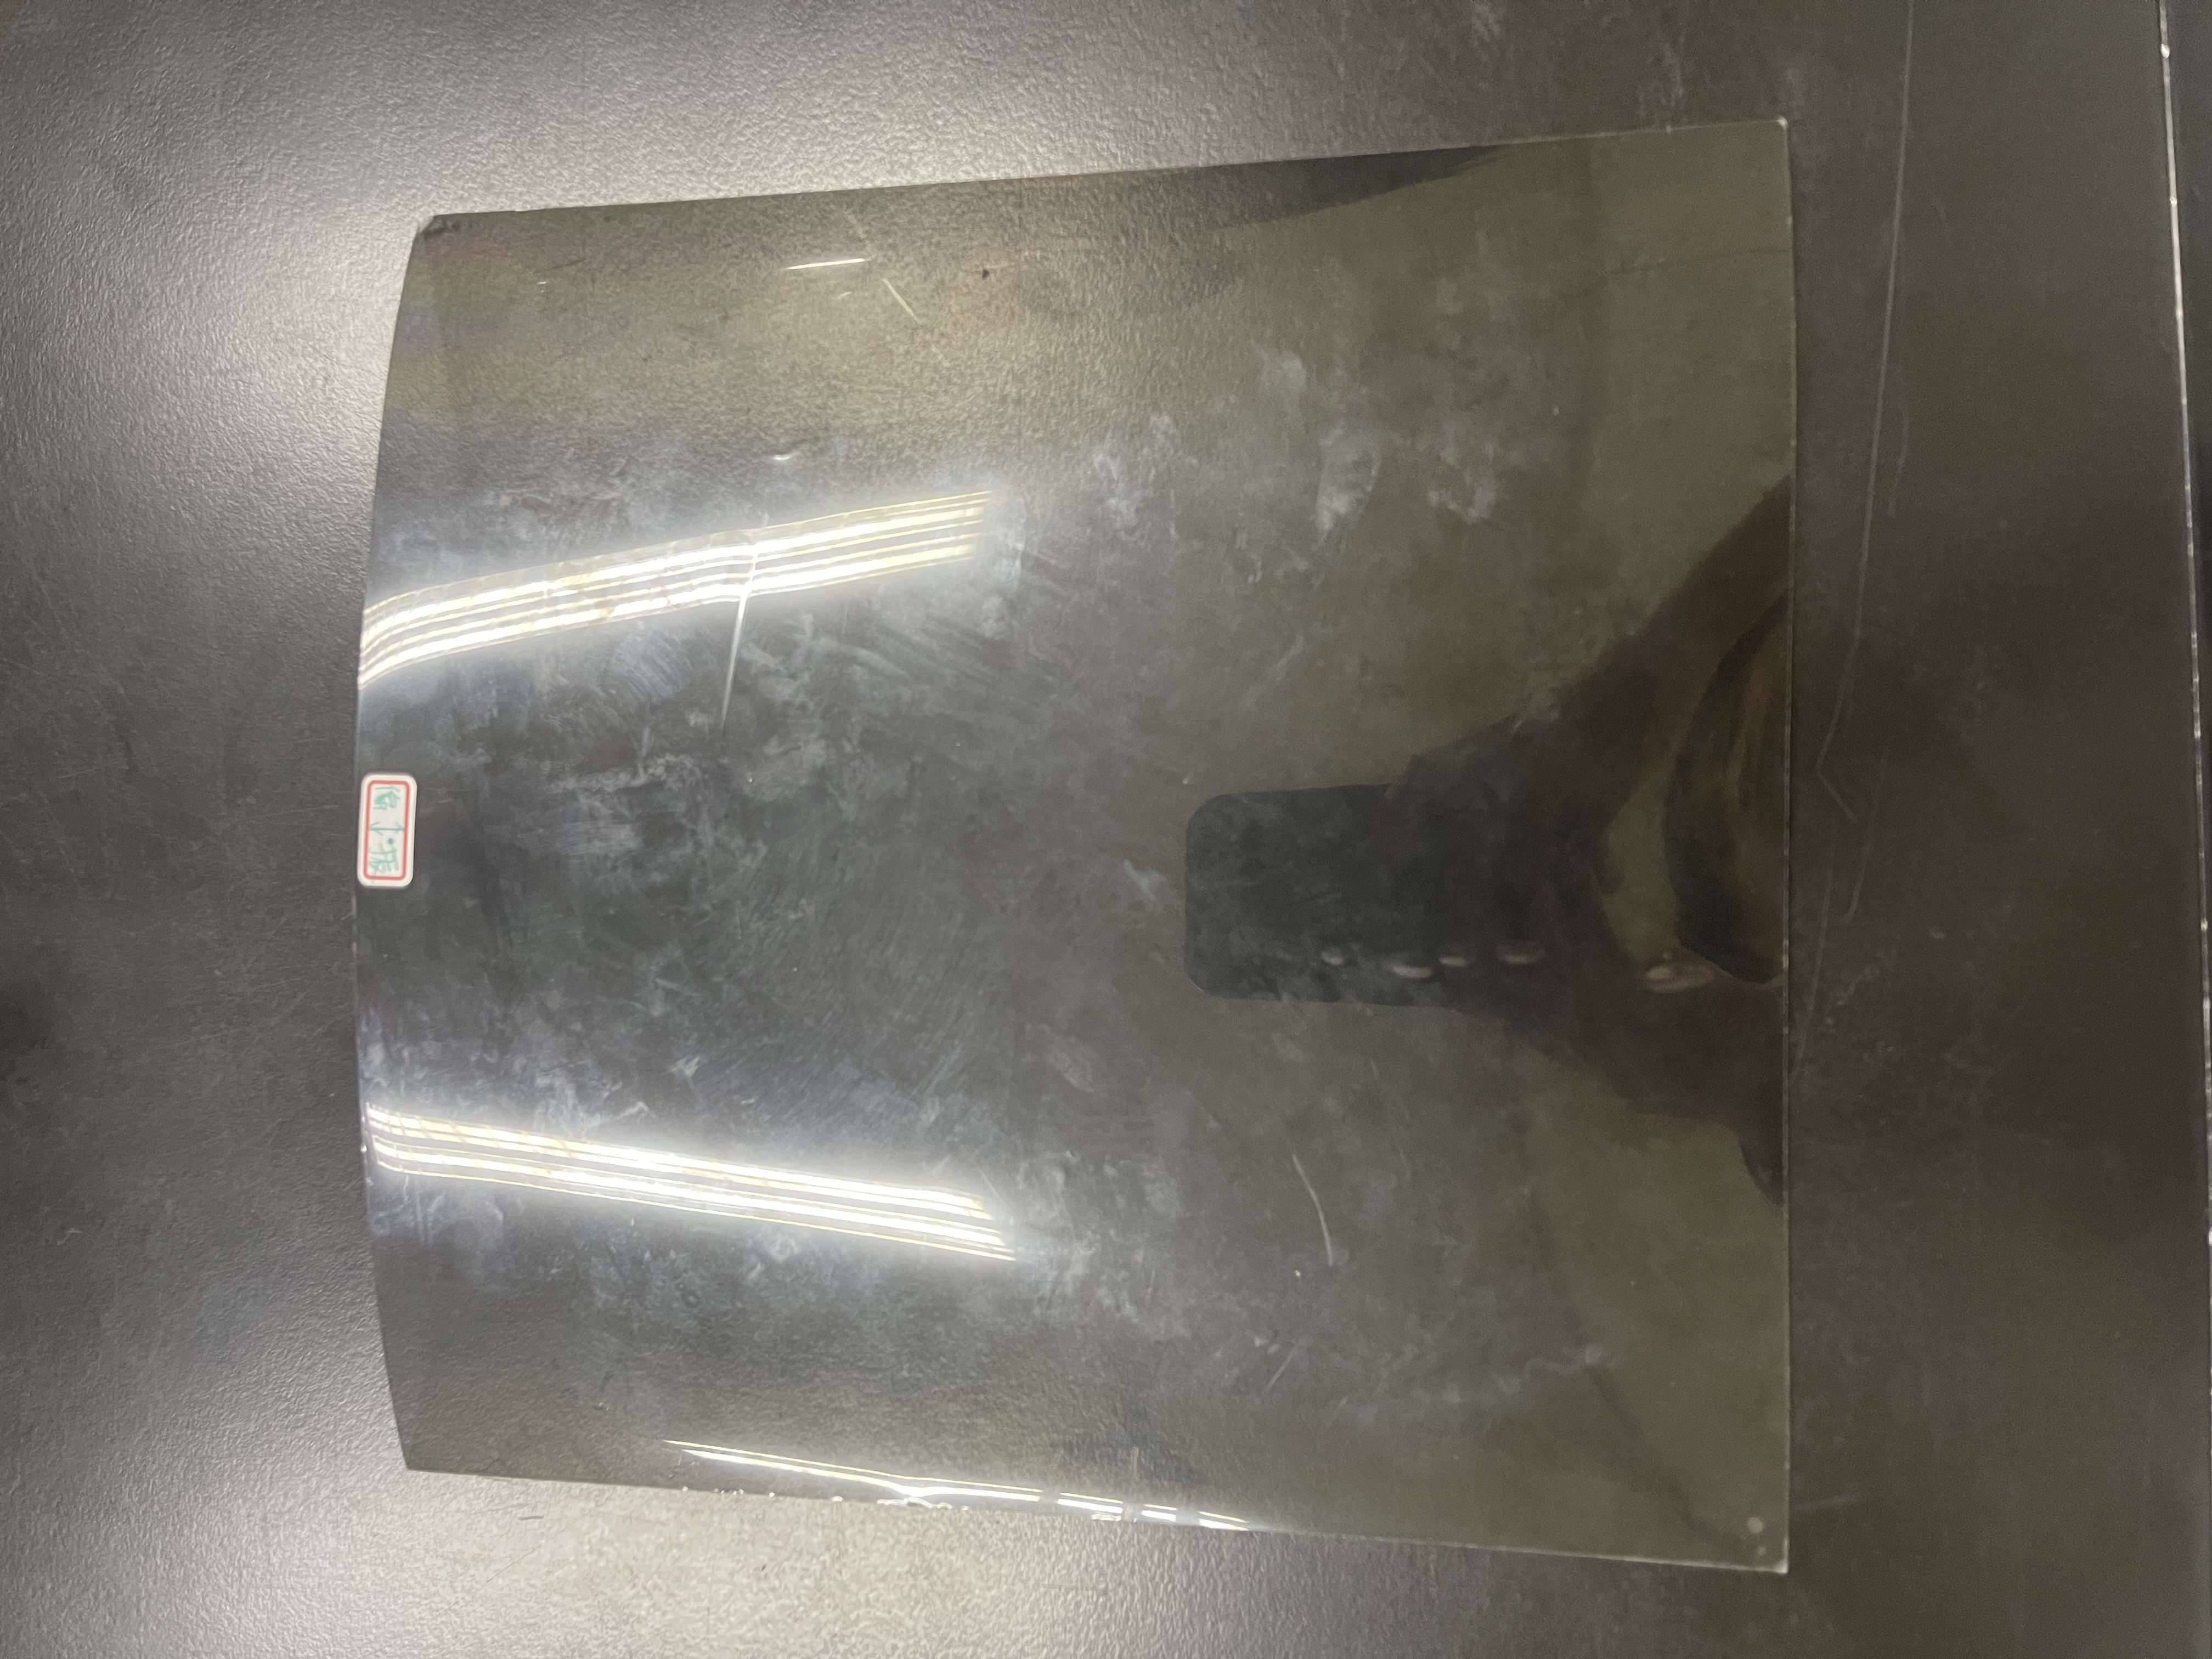
\includegraphics[width=3cm, align=c]{image/偏振片.jpg} & 
        \centering 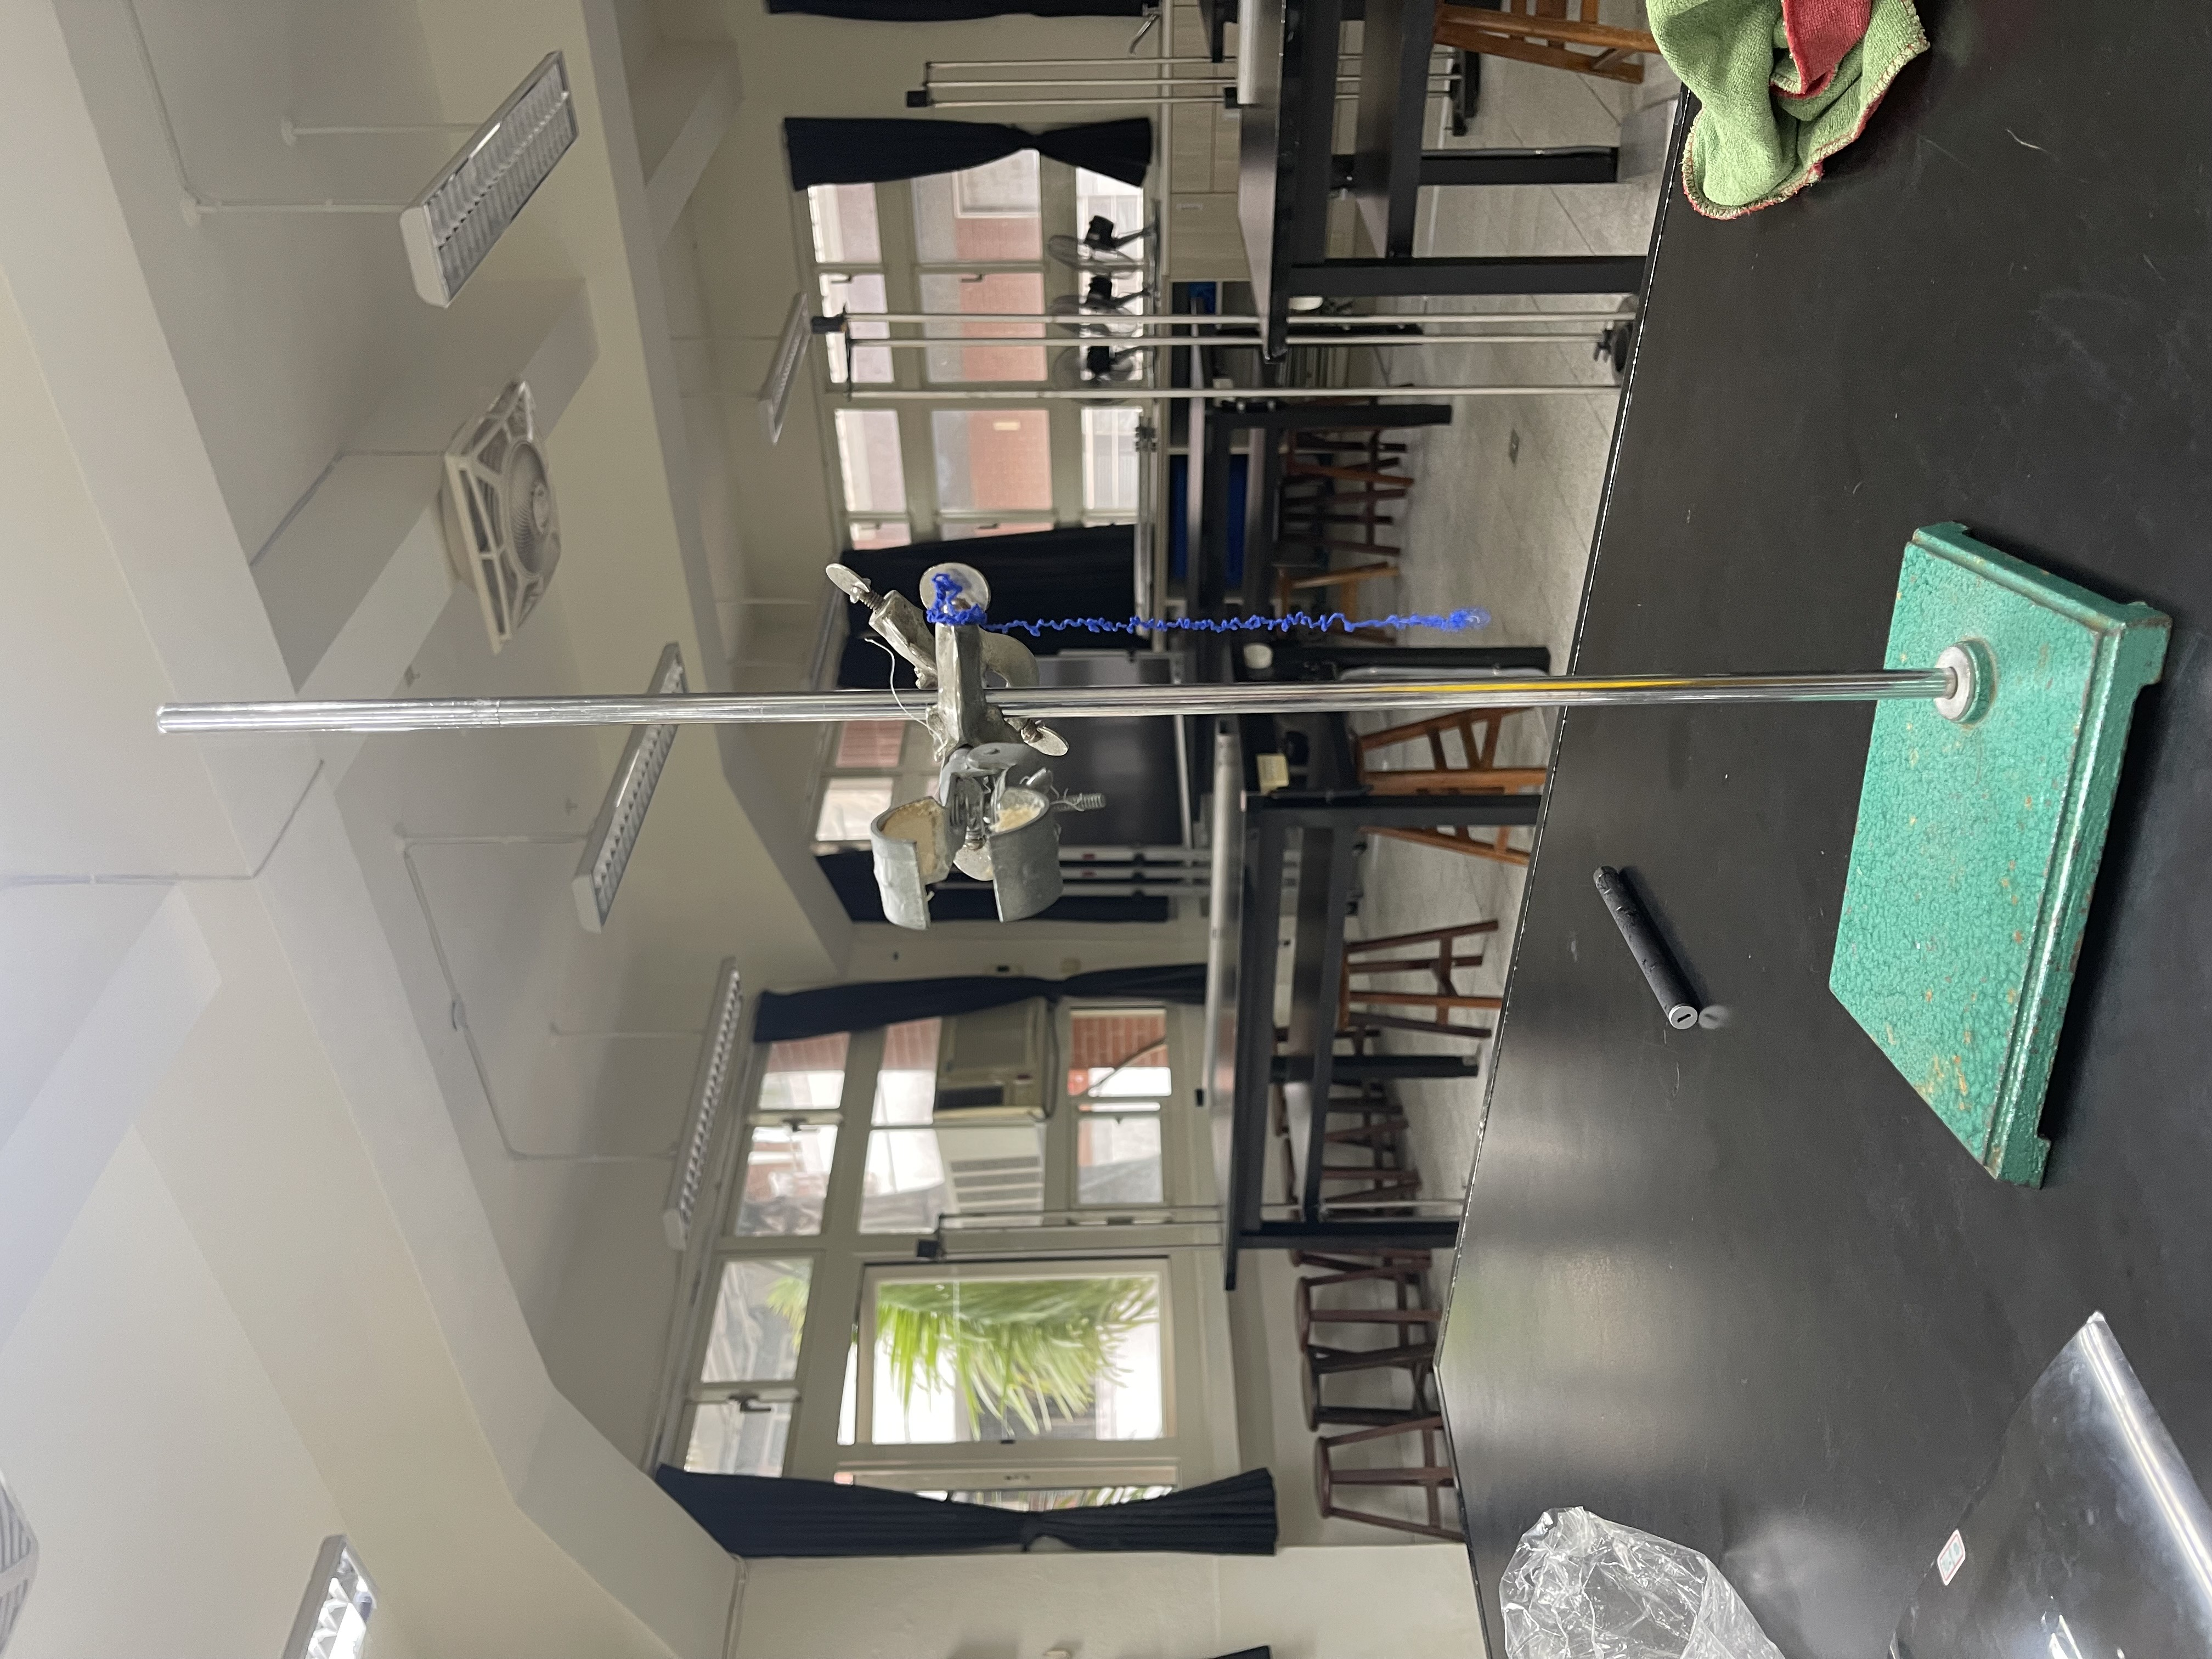
\includegraphics[width=3cm, align=c]{image/角度測量 架子.jpg} \tabularnewline 
        \hline

    \end{tabular}
\end{table}

\subsubsection*{說明}
\begin{enumerate}
    \item 無偏振雷射筆: 任意角度皆有偏振的雷射筆，用於提供入射光
    \item 偏振片: 線偏振偏振片
    \item 支撐架: 固定雷射筆使其入射角維持在布魯斯特角
\end{enumerate}


\subsection*{四、軟體使用}
\begin{table}[H]
    \setlength{\extrarowheight}{1pt}
    \centering
    
    \begin{tabular}{|m{2cm}|m{3cm}|m{3cm}|m{3cm}|}
        \hline
        \centering 名稱 & \centering Python 3.12 & \centering miepython & \centering 自製蒙地卡羅程式 \tabularnewline \hline
        \centering 圖片 & 
        \centering 
\includegraphics[width=2.3cm, align=c]{image/python.jpg} & 
        \centering 
\includegraphics[width=3cm, align=c]{image/miepython.png} & 
        \centering 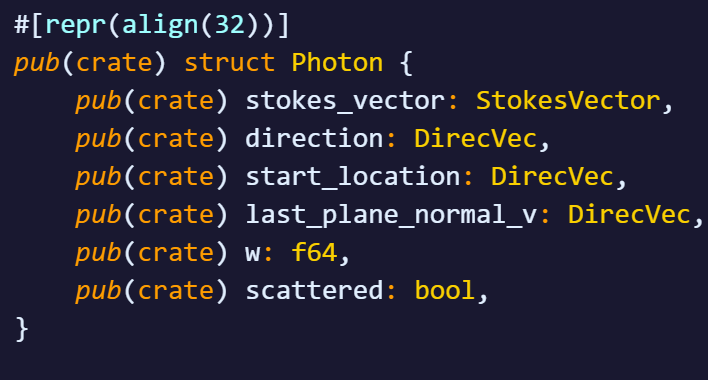
\includegraphics[width=3cm, align=c]{image/蒙地卡羅.png} \tabularnewline 
        \hline

        \centering 名稱 & \centering LEGO EV3 & \centering  rustc 1.98.0 &  \tabularnewline \hline
        \centering 圖片 & 
        \centering 
\includegraphics[width=2.5cm, align=c]{image/ex3_logo.jpg} & 
        \centering 
\includegraphics[width=2.5cm, align=c]{image/rust.png} & \tabularnewline 
        \hline
    \end{tabular}
\end{table}
\subsubsection*{說明}
\begin{itemize}
    \item Python 3：數據處理，包括角度切割、空白扣除、計算 $C$ 與不確定度。
    \item miepython：計算 Mie 散射效率 $Q_{\mathrm{sca}}$、異向性參數 $g$ 與相位函數。
    \item 自製蒙地卡羅程式：模擬多重散射。
    \item LEGO MINDSTORMS EV3 官方軟體：控制旋轉臂每 $1^\circ$ 停留量測。
    \item Rust：撰寫序列埠監測程式並儲存感測資料。
\end{itemize}


\section*{參、研究過程或方法}
% 研究過程與方法
\subsection*{一、研究架構}
本研究分為三個部分：
\begin{enumerate}
\item 建立多角度光散射量測系統與數據處理流程；
\item 量測兩種粒徑的聚苯乙烯微球懸浮液在 $\tau=0.5$ 至 $8$ 時的兩角強度比 $C$；
\item 以蒙地卡羅模擬計算相同條件下的角度分布與 $C$，並和實驗比較。
\end{enumerate}

\subsection*{二、米氏散射與異向性參數}
% 移至附錄
米氏散射描述在介質折射率為 $n$ 的空間中，波長為 $\lambda$ 的光線進入一粒徑為$d$的粒子，若符合 
\begin{equation}
    \frac{2 \pi d n}{\lambda} \approx 1
\end{equation}
則會呈現散射強度隨散射角度產生變化，符合
\begin{align}
    \mathbf{E}_s &= \sum_{n=1}^{\infty} E_n \left( i a_n \mathbf{N}^{(3)}_{e1n} - b_n \mathbf{M}^{(3)}_{o1n} \right), & \mathbf{H}_s &= \frac{k}{\omega\mu} \sum_{n=1}^{\infty} E_n \left( i b_n \mathbf{N}^{(3)}_{o1n} + a_n \mathbf{M}^{(3)}_{e1n} \right) \\
    \mathbf{E}_1 &= \sum_{n=1}^{\infty} E_n \left( c_n \mathbf{M}^{(1)}_{o1n} - i d_n \mathbf{N}^{(1)}_{e1n} \right), & \mathbf{H}_1 &= -\frac{k_1}{\omega\mu_1} \sum_{n=1}^{\infty} E_n \left( d_n \mathbf{M}^{(1)}_{e1n} + i c_n \mathbf{N}^{(1)}_{o1n} \right)
\end{align}
其中 $\mathbf{N}$、$\mathbf{N}$ 為
\begin{align}
    \mathbf{M}_{o1n} &= \cos\phi\, \pi_n z_n(\rho)\, \mathbf{e}_{\theta} - \sin\phi\, \tau_n z_n(\rho)\, \mathbf{e}_{\phi}\\
    \mathbf{M}_{e1n} &= -\sin\phi\, \pi_n z_n(\rho)\, \mathbf{e}_{\theta} - \cos\phi\, \tau_n z_n(\rho)\, \mathbf{e}_{\phi} \\
    \mathbf{N}_{e1n} &= \cos\phi\, n(n+1)\sin\theta\, \pi_n \frac{z_n(\rho)}{\rho}\, \mathbf{e}_r + \cos\phi\, \tau_n \frac{\left[\rho z_n(\rho)\right]'}{\rho}\, \mathbf{e}_{\theta} - \sin\phi\, \pi_n \frac{\left[\rho z_n(\rho)\right]'}{\rho}\, \mathbf{e}_{\phi} \\
    \mathbf{N}_{o1n} &= \sin\phi\, n(n+1)\sin\theta\, \pi_n \frac{z_n(\rho)}{\rho}\, \mathbf{e}_r + \sin\phi\, \tau_n \frac{\left[\rho z_n(\rho)\right]'}{\rho}\, \mathbf{e}_{\theta} + \cos\phi\, \pi_n \frac{\left[\rho z_n(\rho)\right]'}{\rho}\, \mathbf{e}_{\phi}
\end{align}
公式中出現的 $\pi,\ \tau,\ z$ 多項式為米氏散射中的中間公式，詳細證明請參閱\hyperlink{subsec:mie}{附錄的米氏方程導證}。
\\
本研究使用 miepython 計算兩種微球的 Mie 參數。雷射真空波長為 $\lambda=632.8\,\mathrm{nm}$，聚苯乙烯與水的折射率分別約為 $n_{\mathrm{PS}}=1.58$、$n_{\mathrm{water}}=1.332$，相對折射率為 $m=n_{\mathrm{PS}}/n_{\mathrm{water}}$。尺寸參數為 $x=2\pi r n_{\mathrm{water}}/\lambda$。計算所得尺寸參數 $x$、散射效率 $Q_{\mathrm{sca}}$ 與異向性參數 $g=\langle\cos\theta\rangle$ 如下：
\begin{center}
\begin{tabular}{cccc}
    \toprule
    粒徑 ($\mu$m) & $x$ & $Q_{\mathrm{sca}}$ & $g$ \\
    \midrule
    0.492 & 3.25 & 0.700 & 0.818 \\
    2.16 & 14.3 & 2.981 & 0.907 \\
    \bottomrule
\end{tabular}
\end{center}
$g$ 越接近 $1$，散射光越集中於前向。

\subsection*{三、穆勒矩陣與斯托克斯向量}
穆勒矩陣與斯托克向量為描述帶偏振的米氏散射方法。
斯托克向量由四項所構成，分別是總光強度$(I)$、水平與垂直線偏振差$(Q)$、正負$45$度線偏振差$(U)$、右旋與左旋圓偏振差$(V)$。
\begin{align}
    \mathbf{S} = {\left[I, Q, U, V\right]}^T
\end{align}
穆勒矩陣為瓊斯矩陣經過克羅內克積後的結果
\begin{align}
    \mathbf{M} = \mathbf{A} \left(\mathbf{J}\otimes\mathbf{J}^*\right) \mathbf{A}^{-1}
\end{align}

\subsection*{四、光學厚度}
光學厚度 $\tau$ 表示光穿過樣品時平均被散射的次數：
\[
\tau = N Q_{sca} \pi r^2 L
\]
其中 $N$ 為粒子數量濃度（個/$\mathrm{cm}^3$；表中顆/mL 數值代入前須除以 $1000$），$Q_{sca}\pi r^2$ 為一顆粒子的散射截面，
$L=1\,\mathrm{cm}$ 為比色槽光徑。$\tau\ll1$ 時大多數光子最多只被散射一次，
散射光的角度分布就是單一粒子的 Mie 相位函數；$\tau$ 增加後，光子被散
射多次，方向逐漸被打亂，角度分布也被「壓平」。光子方向被打亂所需的距離
，約為平均自由徑的 $\frac{1}{1 - g}$ 倍，稱為傳輸平均自由徑。g 越大，
需要的距離越長，因此在同一個 $\tau$ 下，大顆粒的角度分布應該被壓平得比
較慢。這就是本研究預期 $C(\tau)$ 會因粒徑而不同的物理依據。
\subsection*{五、獨立散射條件}
本研究最濃樣品的粒子平均間距約為粒徑的 $11$ 倍；粒子表面間隙與水中波長之比，對 $0.492\,\mu\mathrm{m}$ 與 $2.16\,\mu\mathrm{m}$ 微球分別約為 $10$ 與 $46$，高於相依散射開始出現的約 $0.3$ 至 $0.5$ 門檻（Baillis \& Sacadura, 2000）。樣品體積分率僅 $0.039\%$，因此將粒子視為獨立散射體；光子可以經歷多次散射，但每次散射仍以單一粒子的 Mie 理論描述。

\subsection*{六、主指標 $C$ 與角度選擇}
本研究以旋轉臂角度作為量測角度。光由比色槽壁射出時會折射，因此臂角與水中的散射角不同；蒙地卡羅模擬納入此折射，實驗與模擬皆以臂角比較。比較不同前向與後向角度組合後，依據數據穩定性、粒徑區別度、對 $\tau$ 的敏感度及與模擬的接近程度，選用
\[
C=\frac{I(30^\circ)}{I(125^\circ)}.
\]
原先使用的 $I(41.8^\circ)/I(138.2^\circ)$ 僅作為對照。

\subsection*{七、樣品配製}
\textbf{(一) 母液數量濃度}\\
兩種聚苯乙烯微球母液的質量濃度皆為 $c=25\,\mathrm{mg/mL}=0.025\,\mathrm{g/mL}$。以聚苯乙烯密度 $\rho\approx1.05\,\mathrm{g/cm^3}$，並假設微球為直徑 $d$ 的球體，母液數量濃度由
\[
N_0=\frac{c}{\rho\,(\pi d^3/6)}
\]
換算，$0.492\,\mu\mathrm{m}$ 微球約為 $3.82\times10^{11}$ 顆/mL，$2.16\,\mu\mathrm{m}$ 微球約為 $4.51\times10^9$ 顆/mL。

\medskip
\noindent\textbf{(二) 稀釋與配製}\\
每槽總體積為 $4000\,\mu\mathrm{L}$，以微量吸管取母液並加去離子水稀釋。各目標光學厚度所需的母液體積及對應數量濃度列於表中。$\tau=1$ 時，兩種微球的數量濃度分別約為 $7.5\times10^8$ 顆/mL 與 $9.2\times10^6$ 顆/mL。母液最少取用 $3.9\,\mu\mathrm{L}$；吸管最小刻度為 $0.1\,\mu\mathrm{L}$，僅刻度造成的相對誤差約為 $3\%$，實際取液誤差可能更大。另以純水配製空白樣品。

\begin{table}[H]
\centering
\caption{不同目標光學厚度的母液用量與數量濃度}
\label{tab:dilution}
\small
\renewcommand{\arraystretch}{1.2}
\begin{tabular}{c|rrrrrr}
    \toprule
    $\tau$ & 0.5 & 1 & 2 & 4 & 6 & 8 \\
    \midrule
    $0.492\,\mu\mathrm{m}$ 母液 ($\mu\mathrm{L}$) & 3.9 & 7.9 & 15.7 & 31.5 & 47.2 & 63.0 \\
    $2.16\,\mu\mathrm{m}$ 母液 ($\mu\mathrm{L}$) & 4.1 & 8.1 & 16.2 & 32.5 & 48.7 & 65.0 \\
    $0.492\,\mu\mathrm{m}$ 數量濃度 ($10^8$ 顆/mL) & 3.8 & 7.5 & 15 & 30 & 45 & 60 \\
    $2.16\,\mu\mathrm{m}$ 數量濃度 ($10^6$ 顆/mL) & 4.6 & 9.2 & 18 & 37 & 55 & 73 \\
    \bottomrule
\end{tabular}
\end{table}

\subsection*{八、實驗量測與數據處理}
\subsubsection*{(一) 量測方式}
\begin{enumerate}
    \item 架設暗室以阻隔環境光，將裝有樣品的方形比色槽放在以雙面膠標示的固定位置。
    \item 調整旋轉臂角度與高度，使直射光剛好照到感測器，並以此位置定為 $0^\circ$。比色槽面向雷射，使槽壁大致垂直於雷射光、但略向前傾，避免反射光直接返回雷射而影響輸出。
    \item 關閉雷射，量測暗室背景與暗讀值；暗室環境亮度確認低於 $0.001\,\mathrm{lux}$。
    \item 開啟雷射後，旋轉臂每次轉動 $1^\circ$ 並停留約 $2$ 秒；含馬達與程式執行時間，每格實測週期約 $2.45$ 秒。旋轉臂由 $0^\circ$ 量至 $140^\circ$ 後返回原位，為一輪；每個樣品量測兩輪，約需 $12$ 分鐘。
    \item 回到 $0^\circ$ 時比對初始讀值，以確認旋轉臂是否回到原位。依 Stokes 定律估算，$2.16\,\mu\mathrm{m}$ 微球在水中的沉降速度約 $0.5\,\mathrm{mm/h}$，一次量測期間沉降約 $0.1\,\mathrm{mm}$，可忽略。
\end{enumerate}
\begin{figure}[H]
    \centering
    % 左邊的照片（寬度設為版面的 48%）
    \begin{subfigure}[b]{0.48\textwidth}
        \centering
        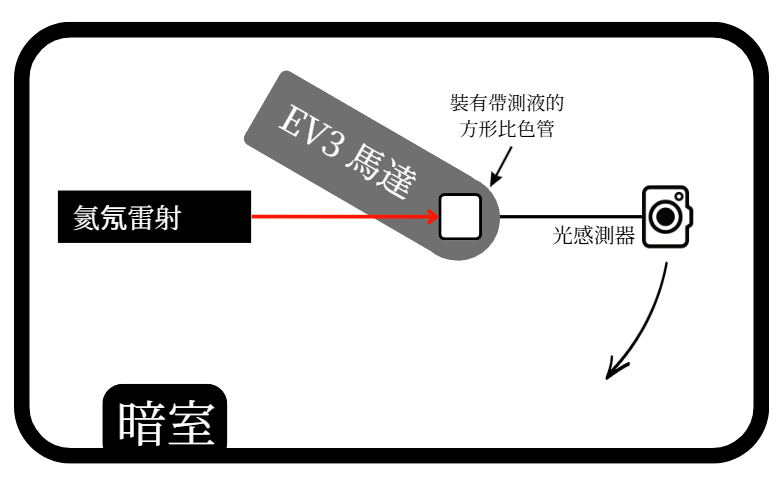
\includegraphics[width=\textwidth]{image/structure.png}
        \caption{裝置實照}\label{fig:left}
    \end{subfigure}
    \hfill 
    \begin{subfigure}[b]{0.48\textwidth}
        \centering
        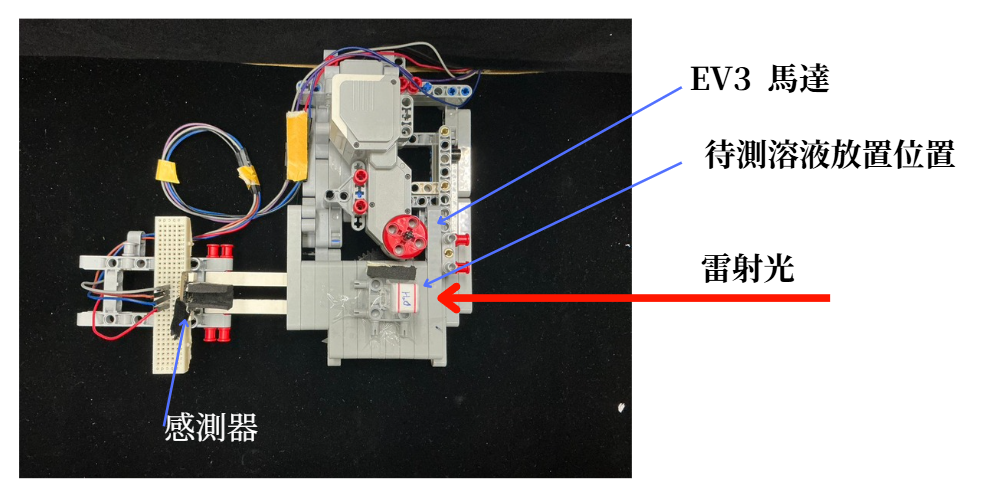
\includegraphics[width=\textwidth]{image/structure_image.png}
        \caption{裝置示意圖}\label{fig:right}
    \end{subfigure}\label{fig:both}
\end{figure}

\subsubsection*{(二) 感測器增益與空白量測}
感測器增益與積分時間由韌體依讀值切換：預設為 HIGH 增益、積分時間 $600\,\mathrm{ms}$；全光譜通道 CH0 低於 $5000$ 時，切換至 MAX 增益、$200\,\mathrm{ms}$，並維持至 CH0 超過 $50000$ 或飽和後才切回 HIGH，以減少頻繁切換。若 HIGH 飽和，則改以 MED 增益、$100\,\mathrm{ms}$ 補讀一筆，該筆不納入分析。依規格書，HIGH 與 MAX 的典型增益分別約為 LOW 的 $400$ 倍與 $9200$ 倍；同型晶片的 HIGH 增益範圍約為 $360$ 至 $440$ 倍，MAX 約為 $8500$ 至 $9900$ 倍（ams-OSRAM AG, 2023）。量測當天於不同時段各量一次純水空白，並量測雷射關閉時的暗讀值。

\subsubsection*{(三) 數據監測方式}
以 Rust 撰寫監測程式，持續讀取 Arduino 的序列埠資料並存成 CSV，以供後續處理。

\subsubsection*{(四) 數據處理}
\begin{enumerate}
    \item 僅保留完整讀值列；剔除飽和讀值、增益切換後的第一筆，以及偏離中位數超過 $4$ 倍穩健標準差的離群值。
    \item 依實測步進週期 $2.45$ 秒推算每個角度格的時間區間，只保留整段曝光都發生在旋轉臂靜止期間的讀值，每格取中位數。
    \item 由每格時間推定臂角（每格 $1^\circ$），再依當天記錄修正角度零點。
    \item 將 HIGH 讀值乘以倍率 $r$，換算為 MAX 等效讀值。依兩種設定的典型增益與積分時間估算，$r=(9200/400)\times(200/600)\approx7.7$；考量晶片個體差異，以旋轉臂靜止且同一格同時有兩種增益讀值的位置，取 MAX 與 HIGH 中位數之比實測，得到 $r=7.48$。此值落在規格範圍內；$30^\circ$ 與 $125^\circ$ 均以 MAX 量得，因此 $C$ 不受此換算影響。
    \item 扣除第二次量測的純水空白，計算淨強度
    \[
        I_{\mathrm{net}}(\theta)=I_{\mathrm{sample}}(\theta)-I_{\mathrm{blank}}(\theta).
    \]
    \item 每輪分別計算 $C=I_{\mathrm{net}}(30^\circ)/I_{\mathrm{net}}(125^\circ)$，再取兩輪平均。
    \item 不確定度取三項平方和開根號：兩輪 $C$ 差的一半、改用另一次純水空白所造成差異的一半，以及角度整體偏移 $\pm0.5^\circ$ 所造成差異的一半。
\end{enumerate}

\subsection*{九、蒙地卡羅模擬}
本研究以蒙地卡羅模擬計算理想條件下（不含雜散光與量測雜訊）的角度分布，作為實驗對照。每顆光子自比色槽入口射入，先依
\[
s=-\frac{\ln\xi}{\mu_s}
\]
前進隨機距離，其中 $\xi$ 為 $0$ 至 $1$ 之間的亂數，$\mu_s$ 為散射係數；碰到微球後，依含粒徑分布的 Mie 相位函數決定新方向，粒徑分布的變異係數分別採用 $0.492\,\mu\mathrm{m}$ 的 $2.1\%$ 與 $2.16\,\mu\mathrm{m}$ 的 $3.1\%$。光子碰到比色槽壁時，依 Fresnel 公式處理水、PMMA（折射率 $1.489$）與空氣界面的反射及透射，包含槽壁內多次反射與全反射；穿出後再依 Snell 定律折射，記錄其落入旋轉臂的 $1^\circ$ 角度格。

每個 $\tau$ 模擬 $5{,}000$ 萬顆光子；光子偏離光束平面超過 $150\,\mathrm{mm}$ 後停止追蹤。模擬假設雷射為非偏振光，旋轉臂半徑取實測值 $110\,\mathrm{mm}$，並以遮光管收光半角 $15.3^\circ$（管長 $11\,\mathrm{mm}$、開口寬 $6\,\mathrm{mm}$）限制感測器收光。每個條件使用 $6$ 組不同亂數種子，取模擬平均值，再以和實驗相同的方式計算 $C$。驗證時，移除比色槽、令 $\tau\to0$ 並只計入單次散射光子，模擬結果與 Mie 理論一致；另以獨立重寫的程式計算六個條件，結果在統計誤差內一致。
\section*{肆、研究結果}
\subsection*{一、兩角強度比隨光學厚度的變化}
本研究以
\[
    C = \frac{I(30^\circ)}{I(125^\circ)}
\]
作為角度分布指標。表一整理兩種粒徑在六個光學厚度下的實驗值與蒙地卡羅模擬值。當 $\tau$ 由 $0.5$ 增加至 $8$，$0.492\,\mu\mathrm{m}$ 微球的實驗 $C$ 由 $12.06$ 降至 $1.92$，$2.16\,\mu\mathrm{m}$ 微球則由 $21.71$ 降至 $3.81$。各光學厚度下，較大粒徑的 $C$ 均較高，約為較小粒徑的 $1.6$ 至 $2.4$ 倍。圖~\ref{fig:C-tau} 上圖為兩者隨 $\tau$ 的變化，下圖為實驗／模擬比值。

\begin{table}[H]
    \centering
    \caption{實驗與蒙地卡羅模擬的兩角強度比 $C$}
    \label{tab:result-c}
    \small
    \renewcommand{\arraystretch}{1.2}
    \begin{tabular}{ccrrr}
        \toprule
        粒徑 ($\mu$m) & $\tau$ & 實驗 $C$ & 模擬 $C$ & 實驗／模擬 \\
        \midrule
        0.492 & 0.5 & $12.06 \pm 0.52$ & 14.02 & $0.86 \pm 0.04$ \\
        0.492 & 1   & $10.85 \pm 0.49$ & 10.34 & $1.05 \pm 0.05$ \\
        0.492 & 2   & $7.47 \pm 0.31$  & 6.32  & $1.18 \pm 0.05$ \\
        0.492 & 4   & $3.93 \pm 0.06$  & 3.14  & $1.25 \pm 0.02$ \\
        0.492 & 6   & $2.62 \pm 0.04$  & 2.00  & $1.31 \pm 0.02$ \\
        0.492 & 8   & $1.92 \pm 0.02$  & 1.49  & $1.29 \pm 0.01$ \\
        \midrule
        2.16  & 0.5 & $21.71 \pm 1.61$ & 25.78 & $0.84 \pm 0.06$ \\
        2.16  & 1   & $17.74 \pm 0.65$ & 20.32 & $0.87 \pm 0.03$ \\
        2.16  & 2   & $15.36 \pm 0.53$ & 13.77 & $1.12 \pm 0.04$ \\
        2.16  & 4   & $9.35 \pm 0.32$  & 7.56  & $1.24 \pm 0.04$ \\
        2.16  & 6   & $6.40 \pm 0.16$  & 4.84  & $1.32 \pm 0.03$ \\
        2.16  & 8   & $3.81 \pm 0.06$  & 3.48  & $1.10 \pm 0.02$ \\
        \bottomrule
    \end{tabular}

    \vspace{0.5ex}
    {\footnotesize 實驗值的 $\pm$ 為合成不確定度（$1\sigma$）；實驗／模擬的 $\pm$ 另合併模擬 $6$ 組亂數種子的標準誤。}
\end{table}

\subsection*{二、角度分布的變化}
隨著 $\tau$ 增加（圖~\ref{fig:Itheta}），前向散射峰逐漸降低，約 $90^\circ$ 附近的低谷也逐漸填平，角度分布趨於平坦。$\tau=8$ 時，$0.492\,\mu\mathrm{m}$ 微球的分布已接近平坦；$2.16\,\mu\mathrm{m}$ 微球仍保有部分前向峰，與其 $C$ 較高的結果一致。

\subsection*{三、實驗與模擬的比較}
蒙地卡羅模擬呈現 $C$ 隨 $\tau$ 增加而下降、且較大粒徑的 $C$ 較高的相同趨勢。當 $\tau\leq 1$，實驗值與模擬值的比值介於 $0.84$ 至 $1.05$；當 $\tau\geq 2$，實驗值比模擬值高約 $10\%$ 至 $32\%$（圖~\ref{fig:C-tau} 下圖）。在 $\tau\geq2$ 時，實驗與模擬整條角度曲線（圖~\ref{fig:abs}）的比值中位數約為 $0.94$ 至 $1.11$，但 $30^\circ$ 附近的實驗強度偏高約 $8\%$ 至 $25\%$；其中 $0.492\,\mu\mathrm{m}$ 微球在 $\tau\geq4$ 時，實驗前向散射部分明顯高於模擬。當 $\tau=0.5$、$1$ 時，整條曲線則整體平移：$0.492\,\mu\mathrm{m}$ 在 $\tau=0.5$、$2.16\,\mu\mathrm{m}$ 在 $\tau=1$ 分別偏高約 $44\%$ 與 $30\%$，$0.492\,\mu\mathrm{m}$ 在 $\tau=1$、$2.16\,\mu\mathrm{m}$ 在 $\tau=0.5$ 分別偏低約 $22\%$ 與 $35\%$。比較時，各條件均沿用同一儀器倍率，未對個別曲線另行調整。

為排除強度倍率的影響，圖~\ref{fig:shape} 將兩者都以 $125^\circ$ 歸一後比較形狀。$\tau\geq4$ 時，$2.16\,\mu\mathrm{m}$ 自 $50^\circ$ 起、$0.492\,\mu\mathrm{m}$ 自 $95^\circ$ 起，形狀比都落在 $1\pm0.1$ 內，偏差集中在前向；$\tau\leq1$ 時，$0.492\,\mu\mathrm{m}$ 在 $80^\circ$ 至 $115^\circ$ 偏高 $20\%$ 至 $41\%$，$2.16\,\mu\mathrm{m}$ 則在 $15^\circ$ 至 $95^\circ$ 間上下起伏。

同一樣品兩輪量測所得 $C$ 的差異多在 $4\%$ 以內，最大約為 $7\%$。本研究的不確定度合併考量兩輪量測差異、替換空白值造成的差異，以及角度整體偏移 $\pm0.5^\circ$ 的影響。

\begin{figure}[H]
    \centering
    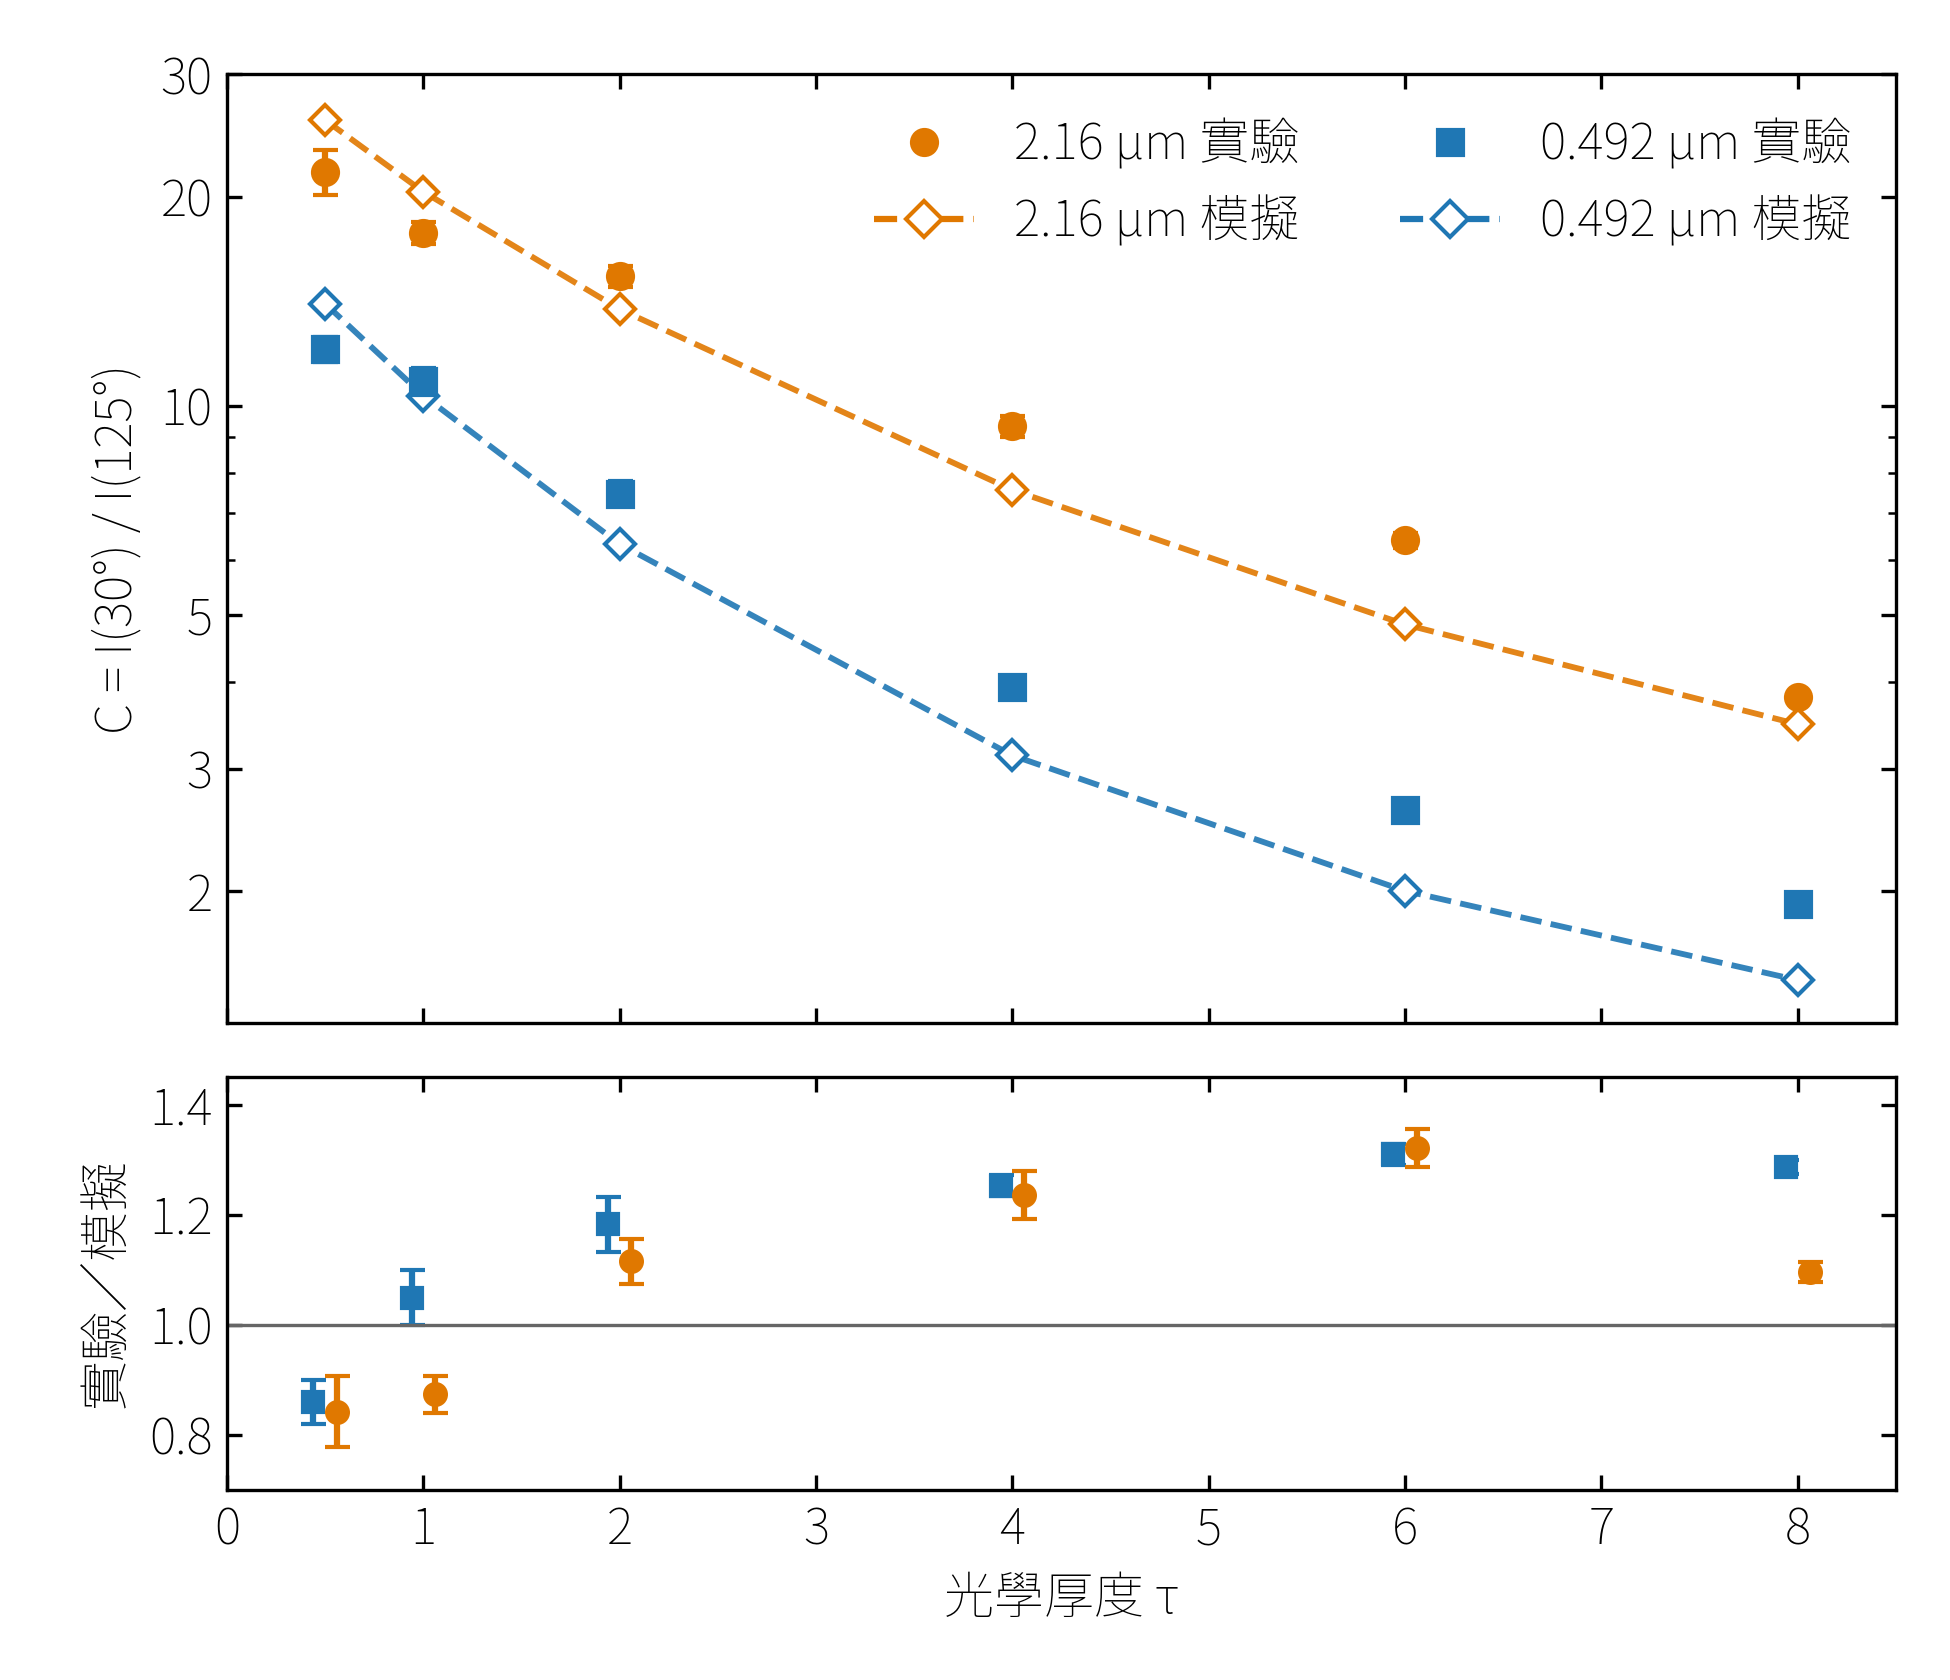
\includegraphics[width=\linewidth]{image/result_C_tau.png}
    \caption{$C$ 隨光學厚度 $\tau$ 的變化。上：實心點為 10 月 24 日實驗值，誤差棒為合成不確定度（$1\sigma$）；空心菱形與虛線為蒙地卡羅模擬（6 組亂數種子平均）；縱軸為對數。下：實驗／模擬比值。}
    \label{fig:C-tau}
\end{figure}

\begin{figure}[H]
    \centering
    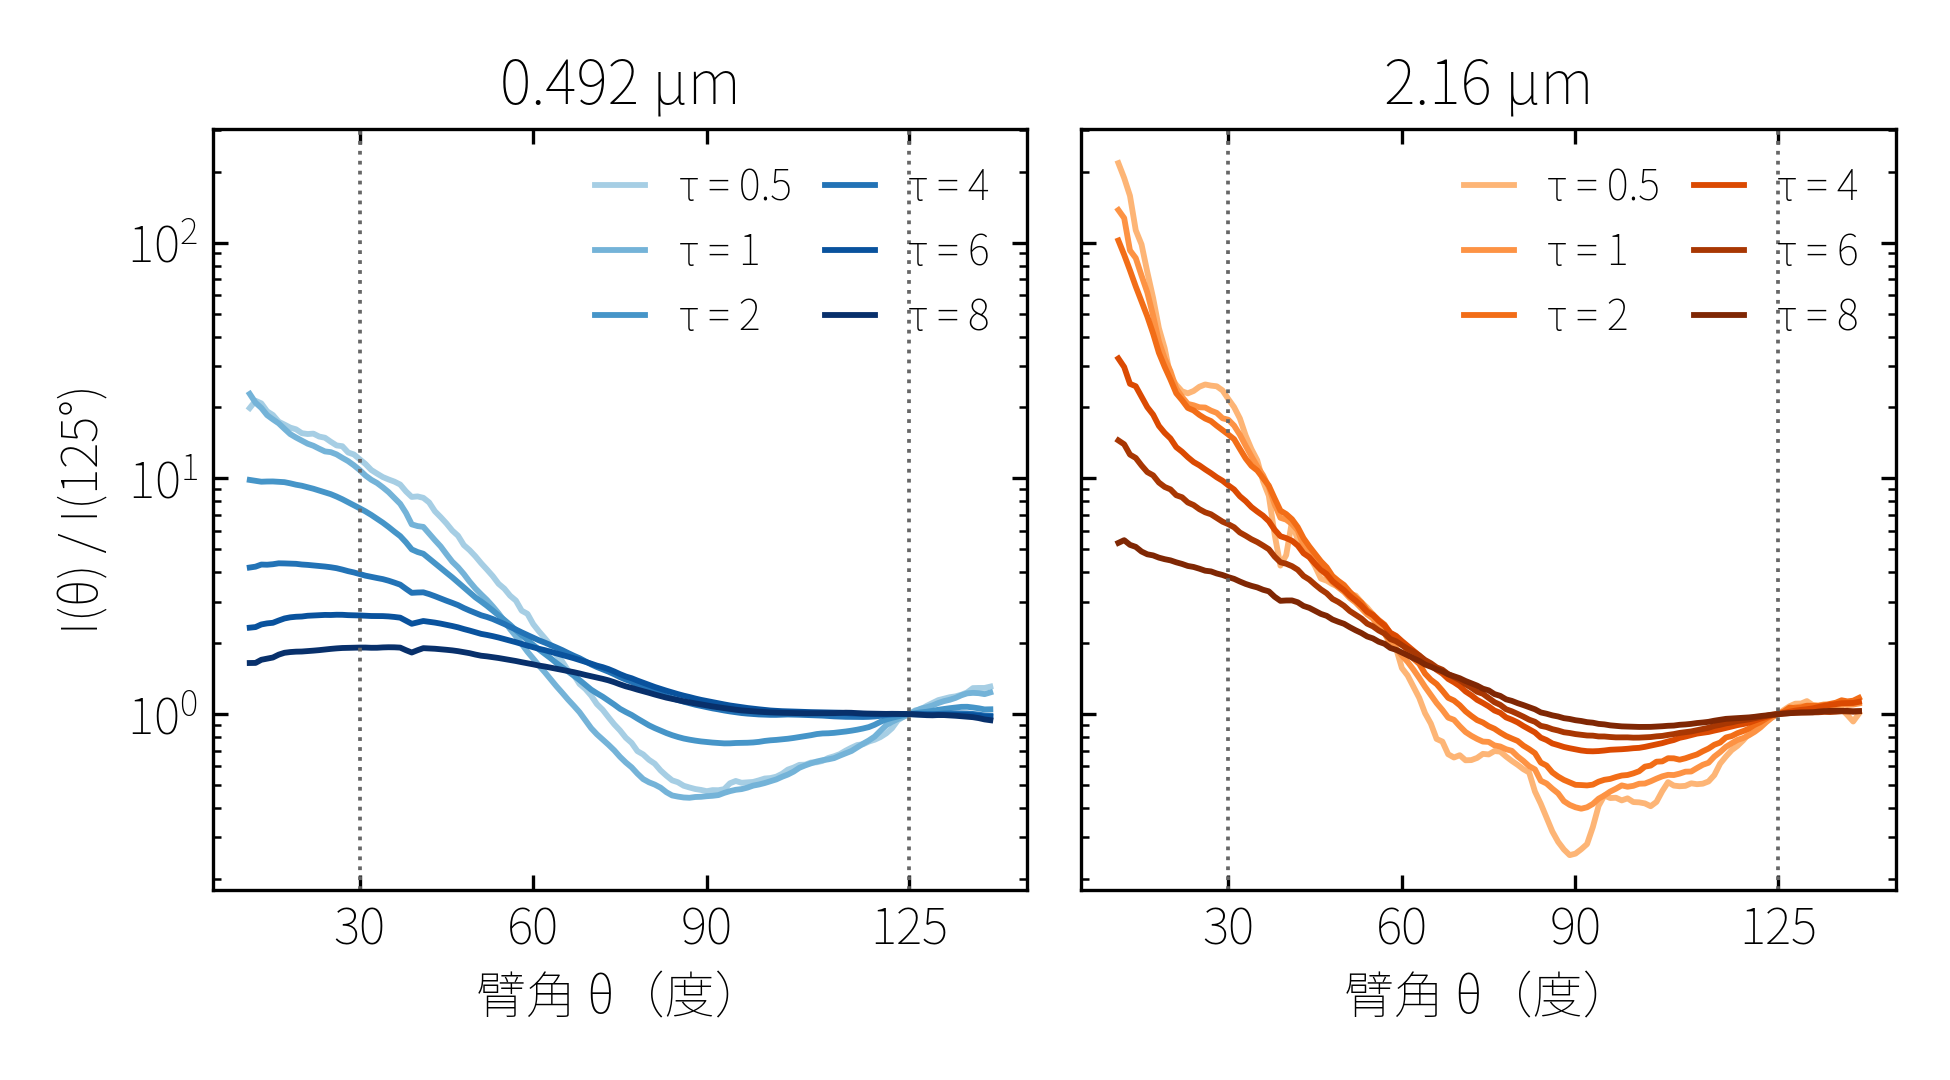
\includegraphics[width=\linewidth]{image/result_Itheta.png}
    \caption{兩種粒徑在不同 $\tau$ 下的實驗角度分布 $I(\theta)/I(125^\circ)$。顏色由淺至深表示 $\tau=0.5$、$1$、$2$、$4$、$6$、$8$；虛線標示 $30^\circ$ 與 $125^\circ$，前者的值即為 $C$。}
    \label{fig:Itheta}
\end{figure}

\begin{figure}[H]
    \centering
    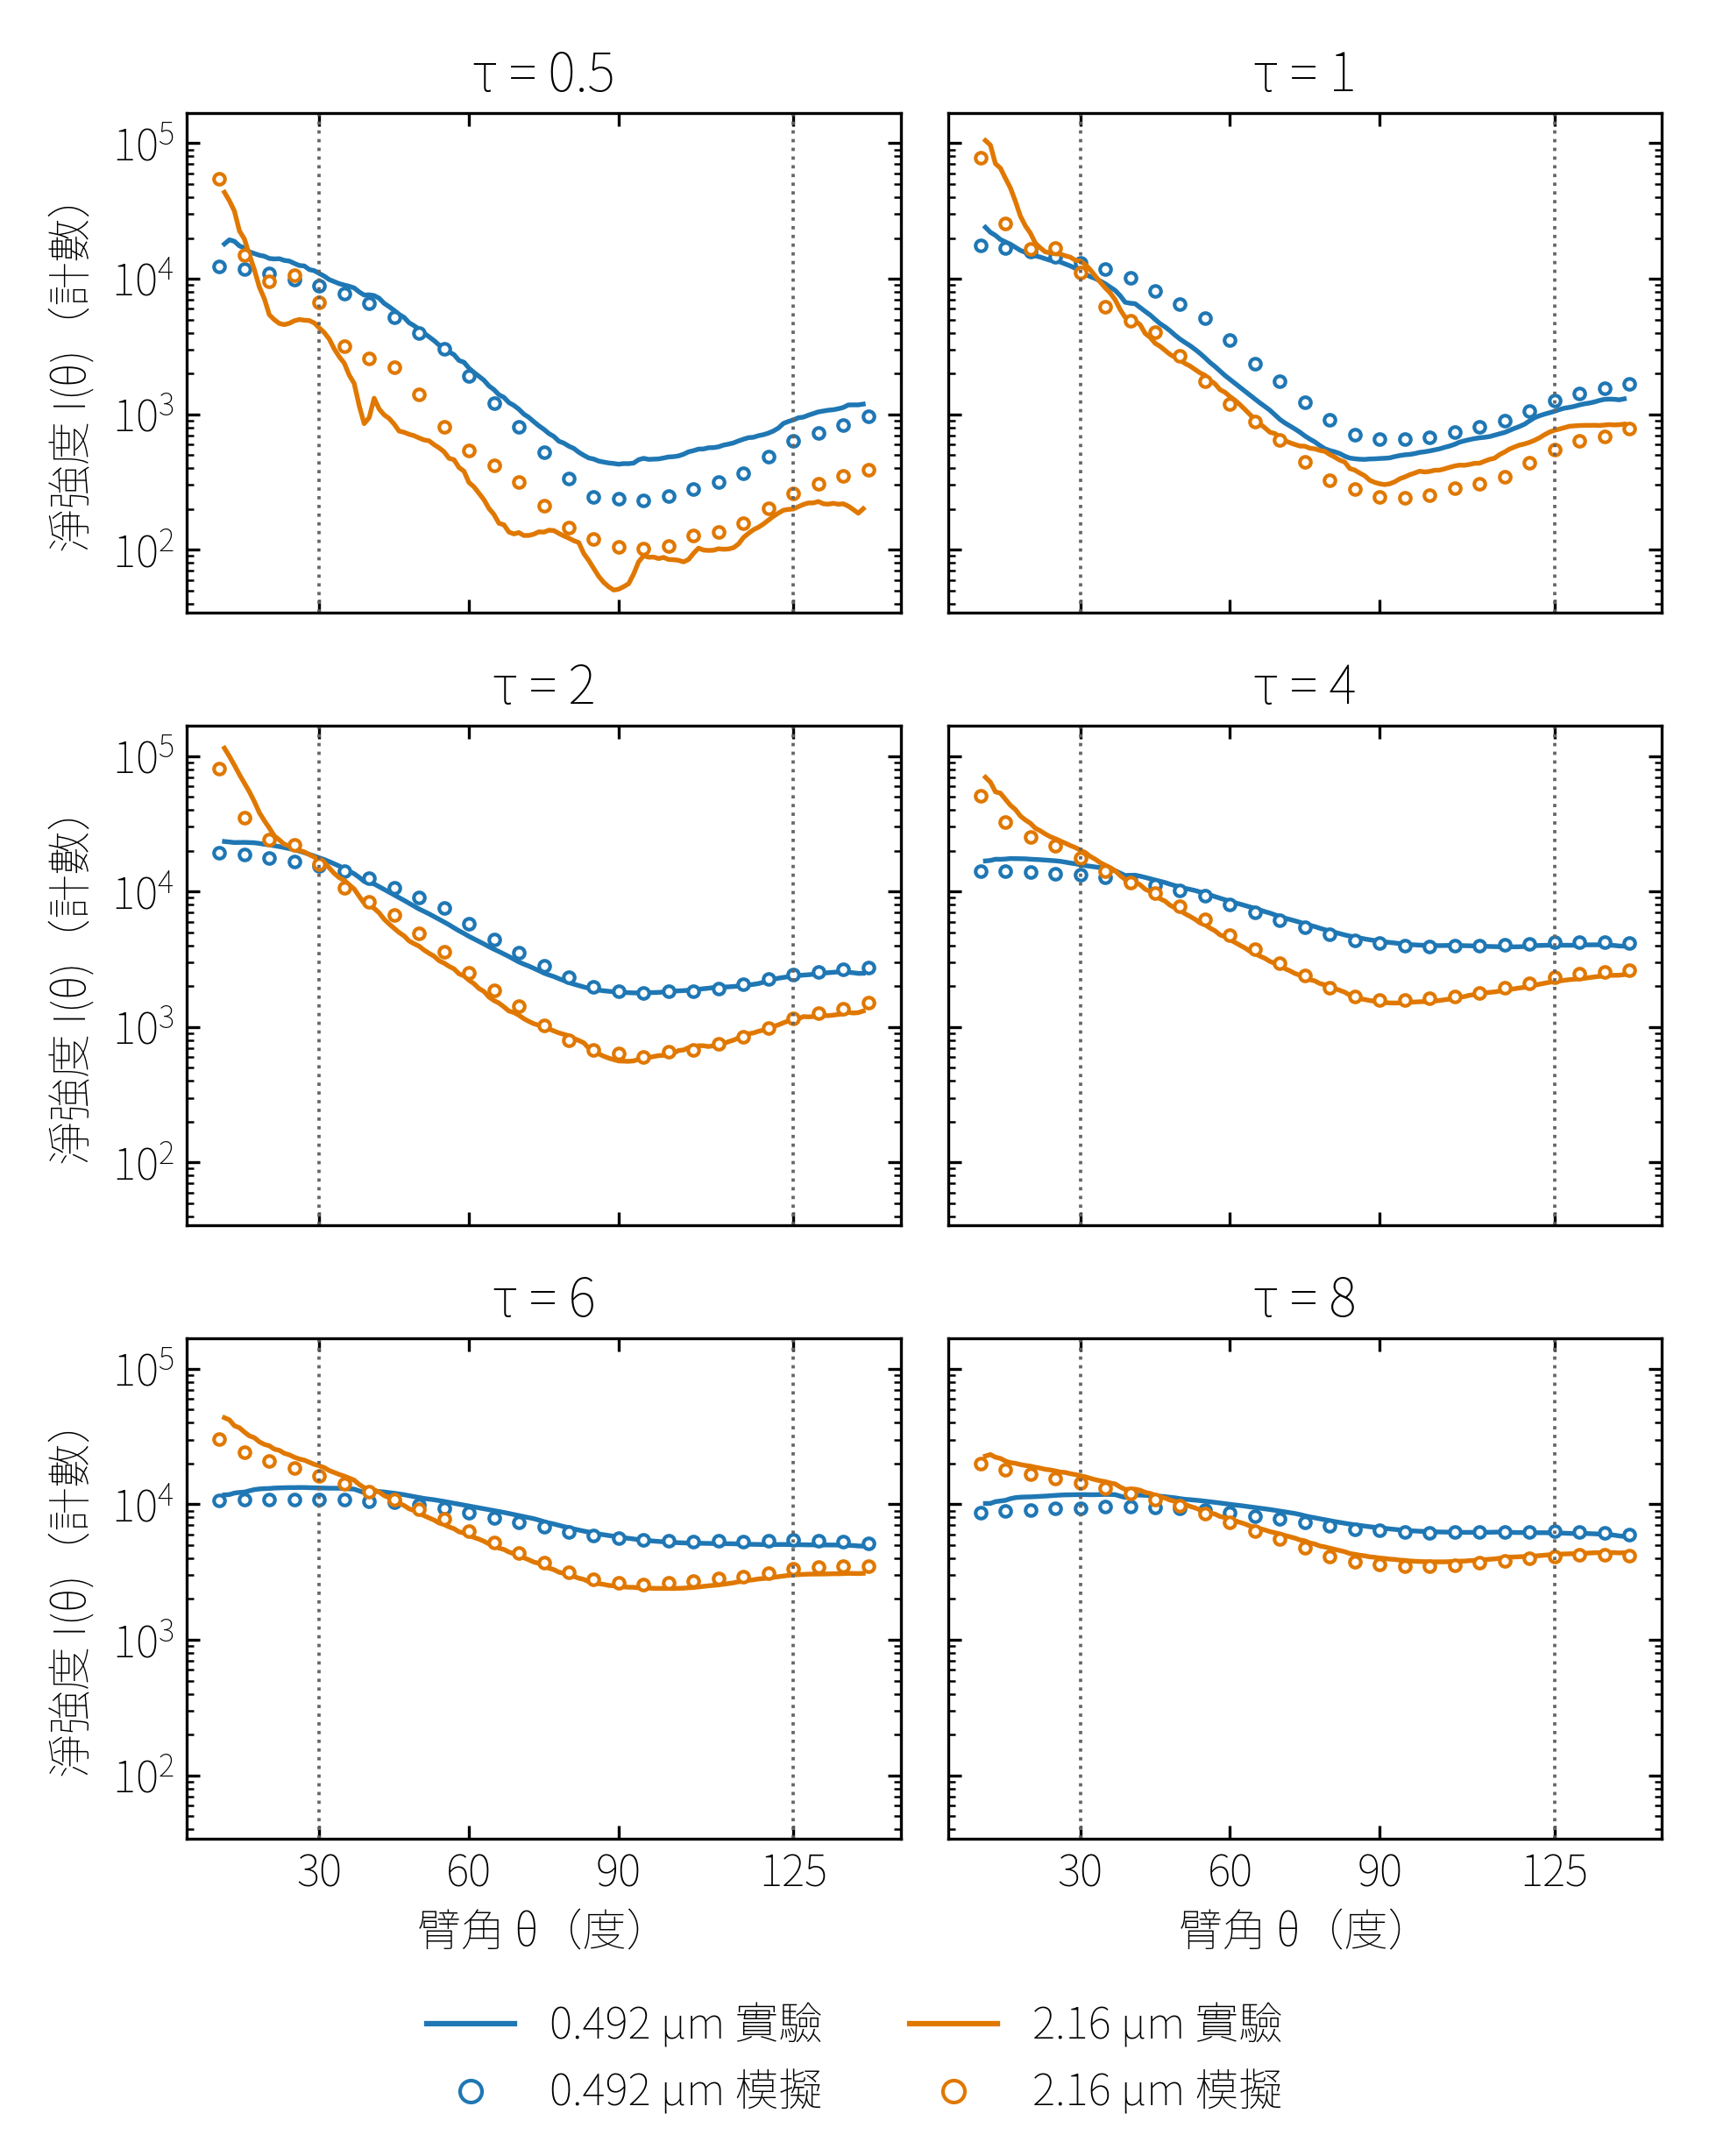
\includegraphics[width=\linewidth]{image/result_abs.png}
    \caption{六個光學厚度下的散射光淨強度 $I(\theta)$。實線為實驗感測器計數，空心圓為蒙地卡羅模擬（$5^\circ$ 一格）乘上共用儀器倍率 $k=2.71\times10^7$；點線標示 $30^\circ$ 與 $125^\circ$。}
    \label{fig:abs}
\end{figure}

\begin{figure}[H]
    \centering
    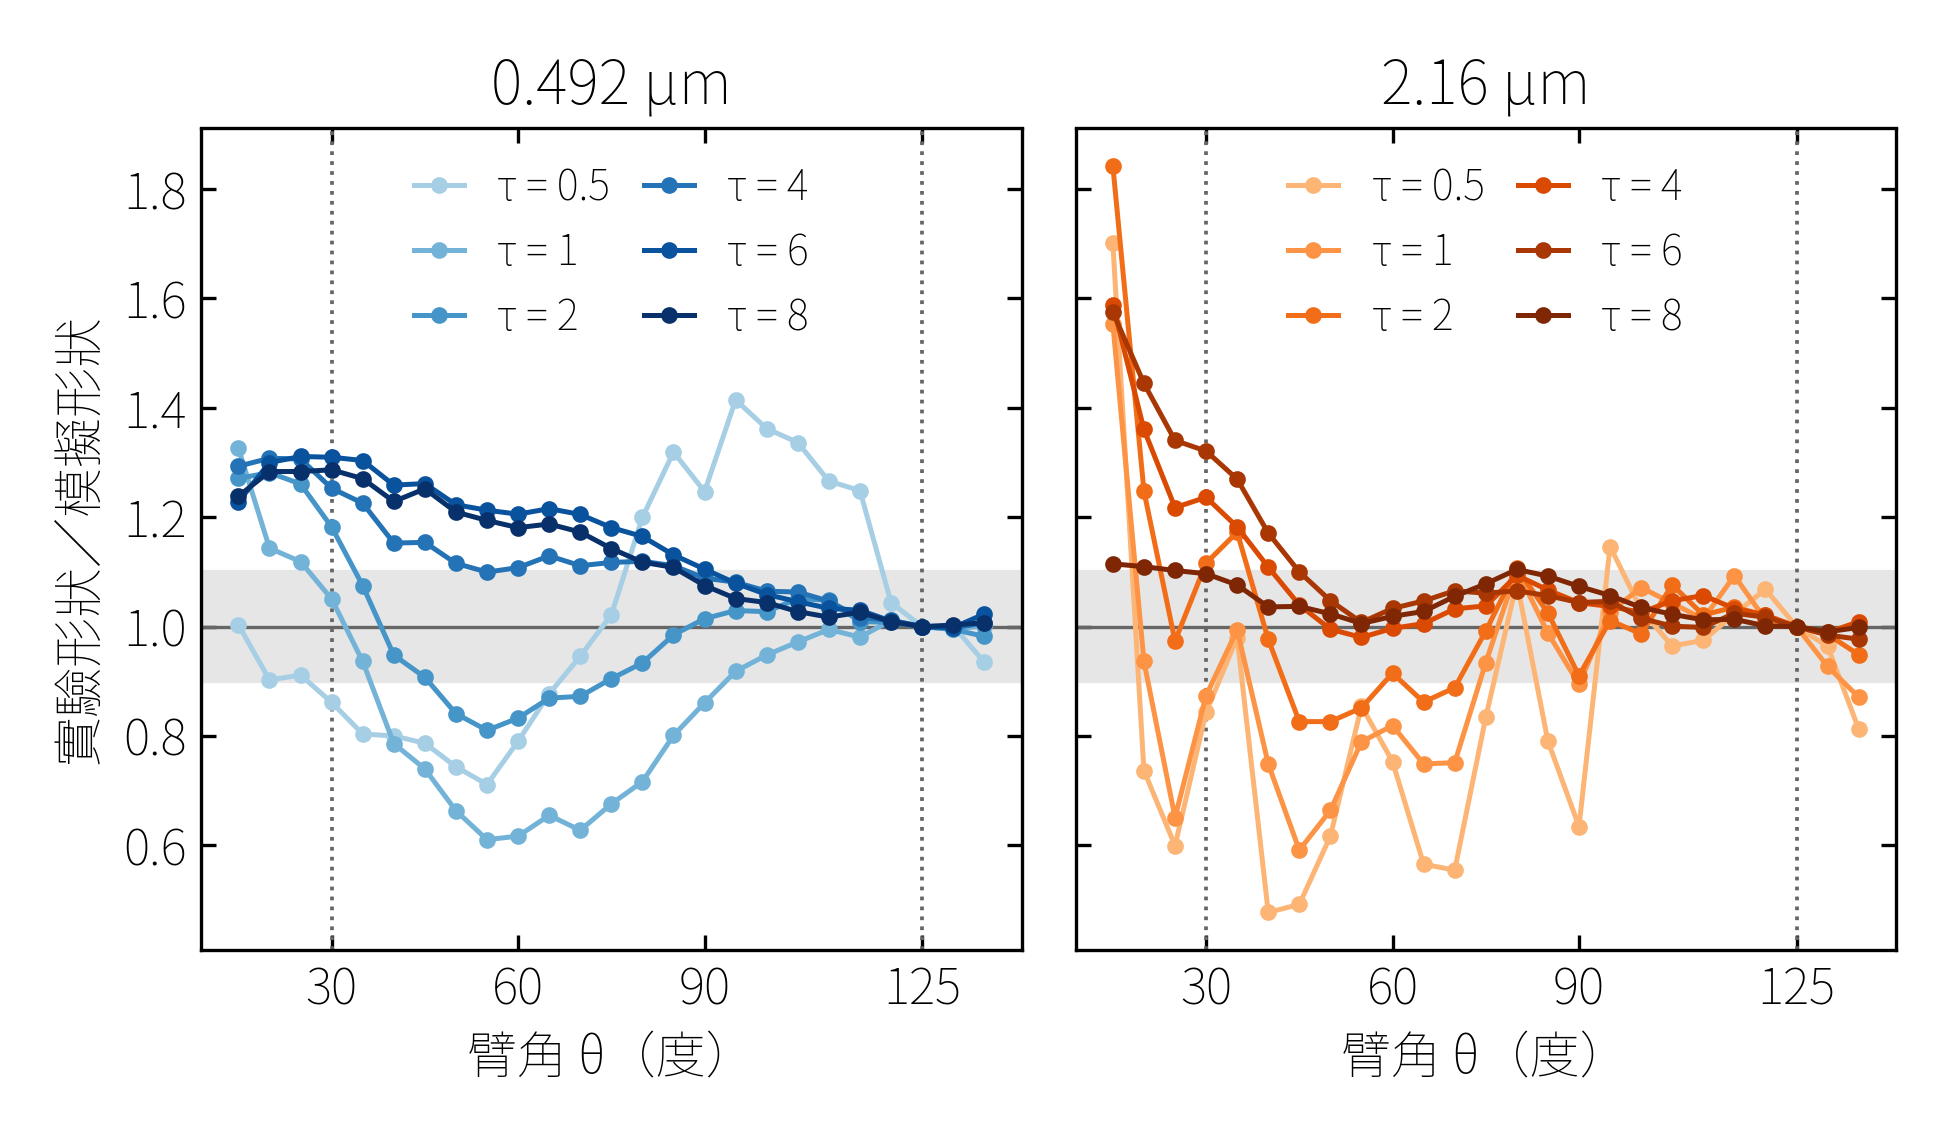
\includegraphics[width=\linewidth]{image/result_shape.png}
    \caption{實驗與模擬角度分布的形狀比 $[I_{\mathrm{exp}}(\theta)/I_{\mathrm{exp}}(125^\circ)]/[I_{\mathrm{MC}}(\theta)/I_{\mathrm{MC}}(125^\circ)]$。$\theta=30^\circ$ 的值即為表~\ref{tab:result-c} 的實驗／模擬比；灰帶為 $1\pm0.1$。}
    \label{fig:shape}
\end{figure}


\section*{伍、討論}
\subsection*{一、$C$ 隨光學厚度下降的原因}
光學厚度較小時，多數光子只經歷一次散射，角度分布仍接近單一粒子的散射分布，前向的 $30^\circ$ 強度遠高於後向的 $125^\circ$ 強度，因此 $C$ 較大。隨著 $\tau$ 增加，光子經歷更多次散射並逐漸失去原有的前進方向，前向峰被壓平，$C$ 隨之下降。

方向記憶消失所需的特徵距離約為傳輸平均自由徑 $l^*=l/(1-g)$，其中 $l$ 為平均自由徑（Pine et al., 1990）。本研究中，$2.16\,\mu\mathrm{m}$ 微球的異向性參數 $g=0.907$，高於 $0.492\,\mu\mathrm{m}$ 微球的 $g=0.818$；前者單次散射的平均偏轉較小，因此在相同 $\tau$ 下，$C$ 下降較慢。

以 $\ln C$ 對 $\tau$ 作直線擬合，實驗斜率在 $2.16\,\mu\mathrm{m}$ 與 $0.492\,\mu\mathrm{m}$ 微球分別為 $-0.224\pm0.007$ 與 $-0.254\pm0.019$；模擬斜率則分別為 $-0.267\pm0.021$ 與 $-0.298\pm0.032$。兩者均支持較大粒徑的下降較慢，但差異僅約 $10\%$ 至 $15\%$。若下降速率只由 $1-g$ 決定，依兩者 $1-g$ 約 $1.95$ 倍的差異，較大粒徑的斜率絕對值應約為另一者的一半；實際結果並非如此。以 $\tau(1-g)$ 作為橫軸時，兩組曲線也未重合。這表示在本研究範圍內，平均異向性參數能說明趨勢方向，卻不足以單獨決定 $C$ 的下降速率；散射相位函數的其他角度細節仍有影響。此範圍的 $\tau(1-g)\leq1.5$，光子尚未進入完全擴散狀態。

\subsection*{二、實驗與模擬的差異}
當 $\tau\geq2$ 時，兩種粒徑的實驗 $C$ 均高於模擬；其中 $0.492\,\mu\mathrm{m}$ 在 $\tau=6$、$8$ 時的實驗／模擬比分別為 $1.31$、$1.29$。樣品管中的背景光應介於完全不扣空白與扣除全部空白兩種極端情形之間；檢查這兩種扣除方式後，差異仍無法消除。可能原因是裝置反光：比色槽周圍的樂高零件與隨旋轉臂移動的線材，被樣品的散射光照亮後再反射進感測器（見參、十一）。圖~\ref{fig:shape} 顯示 $\tau\geq4$ 時偏差集中在前向，與此機制的方向一致。純水空白在臂角約 $40^\circ$ 有一個窄峰，對應線材橫過出射光束的位置，表示線材確實會被照到；但此峰僅約 $700$ 至 $1000$ 計數，遠小於 $2.16\,\mu\mathrm{m}$ 在 $\tau=4$、$6$ 時前向多出的約 $2500$ 至 $5900$ 計數，因此線材應只占一部分，其餘可能來自距比色槽更近的樂高零件。兩者的貢獻需以分步遮黑逐項量測：先包黑線材，再於管座與底座貼上黑絨布。

\subsection*{三、單一兩角強度比的限制}
雖然相同 $\tau$ 下較大粒徑的 $C$ 較高，兩種粒徑的 $C$ 數值範圍仍互有重疊。例如，$0.492\,\mu\mathrm{m}$ 在 $\tau=0.5$ 時的 $C$ 約為 $12.1$，也可能對應到較大粒徑在較高光學厚度時的數值。原稿列出的 12 個樣品中有 9 個，存在不同粒徑與不同 $\tau$ 得到相同 $C$ 的情形。因此，單一 $C$ 無法同時唯一決定粒徑與濃度；若要由 $C$ 推估濃度，需先知道粒徑，或加入其他獨立量測資訊。

\subsection*{四、未來工作}
\begin{enumerate}
    \item 每個濃度配製多管並重複量測，以評估配製誤差及樣品放置時間的影響。
    \item 量測雷射偏振方向與光束位置，並在模擬中納入液面及比色槽底部，釐清 $\tau\geq2$ 時實驗值高於模擬值的原因。
    \item 建立 $C$ 隨 $\tau$ 變化的經驗關係式，在粒徑已知時由 $C$ 反推光學厚度與濃度。
    \item 結合兩組以上角度比，或加入單一角度強度，評估粒徑未知時同時估算粒徑與濃度的可行性。
    \item 探討能否利用 $C$ 判斷單一角度強度位於濃度響應曲線峰值的哪一側，改善單角度讀值的濃度判讀。
    \item 擴大樣品範圍，加入更多粒徑、聚乙烯（PE）、聚對苯二甲酸乙二酯（PET）、混合粒徑及不規則形狀微塑膠，檢驗方法適用範圍及 $C$ 下降速率與 $g$ 的關係。
    \item 朝低成本、可於現場快速估算水中微塑膠粒徑與濃度的量測裝置發展。
\end{enumerate}


\section*{陸、結論}
\begin{enumerate}
    \item 本研究以 He-Ne 雷射、TSL2591 光感測器與樂高旋轉臂建立低成本多角度散射量測系統；同一樣品兩輪量測所得 $C$ 的差異多在 $4\%$ 以內。
    \item 在 $\tau=0.5$ 至 $8$ 的範圍內，$C=I(30^\circ)/I(125^\circ)$ 隨光學厚度增加而下降；相同 $\tau$ 下，$2.16\,\mu\mathrm{m}$ 微球的 $C$ 約為 $0.492\,\mu\mathrm{m}$ 微球的 $1.6$ 至 $2.4$ 倍，顯示兩角強度比在單次散射至多重散射的過渡範圍仍保有粒徑資訊。
    \item $2.16\,\mu\mathrm{m}$ 微球的 $C$ 下降較慢，方向上符合較高 $g$ 所代表的較長傳輸平均自由徑；但下降速率差距僅約 $10\%$ 至 $15\%$，顯示 $C$ 仍受完整散射角度分布影響。
    \item 蒙地卡羅模擬重現了 $C$ 隨 $\tau$ 下降及粒徑差異的趨勢。當 $\tau\leq1$ 時，實驗與模擬比值為 $0.83$ 至 $1.05$；當 $\tau\geq2$ 時，實驗值高於模擬約 $10\%$ 至 $33\%$。前向角附近線材反射是可能原因之一，仍待驗證。
\end{enumerate}


\section*{柒、參考文獻資料}
\sloppy
\begin{enumerate}[label={}, leftmargin=2em, itemsep=0.6em]
    \item ams-OSRAM AG. (2023). \textit{TSL2591 light-to-digital converter} (Version 3-00) [Data sheet]. \url{https://web.physics.ucsb.edu/~phys126/lipman/handouts/datasheets/ams_tsl2591.pdf}
    \item Baillis, D., \& Sacadura, J.-F. (2000). Thermal radiation properties of dispersed media: Theoretical prediction and experimental characterization. \textit{Journal of Quantitative Spectroscopy and Radiative Transfer, 67}(5), 327--363. \url{https://doi.org/10.1016/S0022-4073(99)00234-4}
    \item Berrocal, E., Sedarsky, D. L., Paciaroni, M. E., Meglinski, I. V., \& Linne, M. A. (2007). Laser light scattering in turbid media Part I: Experimental and simulated results for the spatial intensity distribution. \textit{Optics Express, 15}(17), 10649--10665. \url{https://doi.org/10.1364/OE.15.010649}
    \item Genc, S., Icoz, K., \& Erdem, T. (2023). Numerical analysis and experimental verification of optical scattering from microplastics. \textit{Royal Society Open Science, 10}(8), 230586. \url{https://doi.org/10.1098/rsos.230586}
    \item Lotfi Choobbari, M., Ciaccheri, L., Chalyan, T., Adinolfi, B., Thienpont, H., Meulebroeck, W., \& Ottevaere, H. (2022). Batch analysis of microplastics in water using multi-angle static light scattering and chemometric methods. \textit{Analytical Methods, 14}(39), 3840--3849. \url{https://doi.org/10.1039/D2AY01215D}
    \item Pine, D. J., Weitz, D. A., Zhu, J. X., \& Herbolzheimer, E. (1990). Diffusing-wave spectroscopy: Dynamic light scattering in the multiple scattering limit. \textit{Journal de Physique, 51}(18), 2101--2127. \url{https://doi.org/10.1051/jphys:0199000510180210100}
\end{enumerate}


\section*{捌、附錄}
% 此為附錄
\subsection*{(一) 米氏散射導證} \hypertarget{subsec:mie}{}
% 米氏散射：推導骨架（完整推導見 Mie (1908) 與 Bohren & Huffman (1983) 第四章）
本附錄只列出推導的骨架與本研究用到的結果，各步驟的完整推導見 \textcite{https://doi.org/10.1002/andp.19083300302} 的原始論文，符號與寫法依 \textcite{bohren1983Absorption} 第四章。

\subsubsection*{(一) 亥姆霍茲方程}
均勻、無源介質中的馬克士威方程式取時諧形式 $e^{-i\omega t}$ 後，電場與磁場皆滿足向量亥姆霍茲方程，且散度為零：
\begin{equation}
    \nabla^2\mathbf{E} + k^2 \mathbf{E} = 0, \qquad \nabla\cdot\mathbf{E}=0, \qquad k^2 = \omega^2 \epsilon \mu .
\end{equation}

\subsubsection*{(二) 球面邊界條件}
在球面 $r=a$ 上，電場與磁場的切向分量連續：
\begin{equation}
    \left(\mathbf{E}_{i} + \mathbf{E}_{s} - \mathbf{E}_{1}\right) \times \mathbf{e}_r = 0, \qquad \left(\mathbf{H}_{i} + \mathbf{H}_{s} - \mathbf{H}_{1}\right) \times \mathbf{e}_r = 0 ,
\end{equation}
其中下標 $i$、$s$、$1$ 分別代表入射場、散射場與球內場。

\subsubsection*{(三) 向量球面波函數}
由滿足純量亥姆霍茲方程的生成函數 $\psi$ 建構
\begin{equation}
    \mathbf{M} = \nabla \times (\mathbf{r} \psi), \qquad \mathbf{N} = \frac{\nabla \times \mathbf{M}}{k},
\end{equation}
兩者皆滿足向量亥姆霍茲方程、散度為零，且互為旋度，因此可用來展開電磁場。$\psi$ 在球座標下分離變數後，角向解為連帶勒讓德函數 $P_n^{\ell}(\cos\theta)$ 與 $\cos\ell\phi$、$\sin\ell\phi$，徑向解為球貝索函數 $z_n(kr)$：球內與入射場取在原點有限的 $j_n$，散射場取向外傳播的球漢克爾函數 $h_n^{(1)}$。平面波入射時只用到 $\ell=1$ 的項，定義角函數
\begin{equation}
    \pi_n = \frac{P_n^1\left(\cos\theta\right)}{\sin\theta}, \qquad \tau_n = \frac{dP_n^1\left(\cos\theta\right)}{d\theta} .
\end{equation}
這些函數在球面上彼此正交，所以展開係數可以由內積直接求出\parencite{bohren1983Absorption}。

\subsubsection*{(四) 場的級數展開}
沿 $+z$ 傳播、沿 $x$ 方向偏振的平面波，由正交關係可得只剩 $\mathbf{M}_{o1n}$ 與 $\mathbf{N}_{e1n}$ 兩組項：
\begin{equation}
    \mathbf{E}_i = \sum_{n=1}^{\infty} E_n \left( \mathbf{M}^{(1)}_{o1n} - i \mathbf{N}^{(1)}_{e1n} \right), \qquad E_n = i^n E_0 \frac{2n+1}{n(n+1)} .
\end{equation}
散射場與球內場的角向依賴和入射場相同，只差待定係數：
\begin{equation}
    \mathbf{E}_s = \sum_{n=1}^{\infty} E_n \left( i a_n \mathbf{N}^{(3)}_{e1n} - b_n \mathbf{M}^{(3)}_{o1n} \right), \qquad
    \mathbf{E}_1 = \sum_{n=1}^{\infty} E_n \left( c_n \mathbf{M}^{(1)}_{o1n} - i d_n \mathbf{N}^{(1)}_{e1n} \right) .
\end{equation}
上標 $(1)$、$(3)$ 分別代表徑向函數取 $j_n$ 與 $h_n^{(1)}$。

\subsubsection*{(五) 散射係數與截面}
把各場代入 (二) 的邊界條件，令尺寸參數 $x = ka$、相對折射率 $m = k_1/k$，並以 Riccati--Bessel 函數 $\psi_n(\rho) = \rho\, j_n(\rho)$、$\xi_n(\rho) = \rho\, h_n^{(1)}(\rho)$ 表示，解得米氏散射係數
\begin{align}
    a_n &= \frac{m\, \psi_n(mx)\, \psi_n^{\prime}(x) - \psi_n(x)\, \psi_n^{\prime}(mx)}{m\, \psi_n(mx)\, \xi_n^{\prime}(x) - \xi_n(x)\, \psi_n^{\prime}(mx)}, \\
    b_n &= \frac{\psi_n(mx)\, \psi_n^{\prime}(x) - m\, \psi_n(x)\, \psi_n^{\prime}(mx)}{\psi_n(mx)\, \xi_n^{\prime}(x) - m\, \xi_n(x)\, \psi_n^{\prime}(mx)} ,
\end{align}
$a_n$、$b_n$ 分別對應第 $n$ 階的電型與磁型多極輻射。將遠場的散射功率對全球面積分，再除以入射強度與幾何截面 $\pi a^2$，得散射效率；由光學定理可得消光效率：
\begin{equation}
    \begin{aligned}
    Q_{sca} &= \frac{2}{x^2} \sum_{n=1}^{\infty}(2n+1)\left(|a_n|^2+|b_n|^2\right), \\
    Q_{ext} &= \frac{2}{x^2} \sum_{n=1}^{\infty} (2n+1)\, \mathrm{Re}\left\{ a_n + b_n \right\} .
    \end{aligned}
    \label{eq:Qsca_proof}
\end{equation}
級數在 $n$ 略大於 $x$ 之後迅速收斂，數值計算通常取 $n_{max} \approx x + 4x^{1/3} + 2$\parencite{bohren1983Absorption}。


\subsection*{(二) 穆勒矩陣與斯托克斯向量}
% 米氏散射：瓊斯矩陣、斯托克斯向量與穆勒矩陣（骨架；完整推導見 Bohren & Huffman (1983) 第二至四章）

\subsubsection*{(六) 遠場與振幅散射矩陣（瓊斯矩陣）}
本節只列出結果，推導見 \textcite{bohren1983Absorption} 第三、四章；瓊斯矩陣的寫法源自 \textcite{jones1941NewCalculus}。

在遠場（$kr \gg x^2$），散射場為橫向的局部平面波。以包含入射方向與散射方向的平面為散射面，將電場分解為平行（$\parallel$）與垂直（$\perp$）於散射面的分量，散射場與入射場的關係為
\begin{equation}
    \begin{pmatrix} E_{s\parallel} \\ E_{s\perp} \end{pmatrix} = \frac{e^{ikr}}{-ikr} \begin{pmatrix} S_2(\theta) & 0 \\ 0 & S_1(\theta) \end{pmatrix} \begin{pmatrix} E_{\parallel i} \\ E_{\perp i} \end{pmatrix} , \label{eq:jones}
\end{equation}
其中振幅散射函數為
\begin{equation}
    S_1(\theta) = \sum_{n=1}^{\infty} \frac{2n+1}{n(n+1)} \left( a_n \pi_n + b_n \tau_n \right), \qquad S_2(\theta) = \sum_{n=1}^{\infty} \frac{2n+1}{n(n+1)} \left( a_n \tau_n + b_n \pi_n \right) . \label{eq:S1S2}
\end{equation}
球對任何通過球心的軸旋轉對稱，因此矩陣的非對角元為零，且 $S_1$、$S_2$ 只與散射角 $\theta$ 有關。$\parallel$ 與 $\perp$ 分量各自乘上 $S_2$、$S_1$；一般 $S_1 \neq S_2$，所以散射會改變偏振態。

\subsubsection*{(七) 斯托克斯向量}
斯托克斯參數由 \textcite{stokes1852Composition} 提出，本節的定義與參考面旋轉依 \textcite{bohren1983Absorption} 第二章。斯托克斯參數定義為
\begin{equation}
    \begin{aligned}
        I &= \langle E_{\parallel} E_{\parallel}^* + E_{\perp} E_{\perp}^* \rangle, \qquad & Q &= \langle E_{\parallel} E_{\parallel}^* - E_{\perp} E_{\perp}^* \rangle \\
        U &= \langle E_{\parallel} E_{\perp}^* + E_{\perp} E_{\parallel}^* \rangle, \qquad & V &= i \langle E_{\parallel} E_{\perp}^* - E_{\perp} E_{\parallel}^* \rangle
    \end{aligned} \label{eq:stokes_def}
\end{equation}
其中 $\langle\cdot\rangle$ 為時間平均，斯托克斯向量為 $\mathbf{S} = (I, Q, U, V)^{T}$；完全偏振光滿足 $I^2 = Q^2 + U^2 + V^2$。若把參考軸繞傳播方向轉動角度 $\alpha$，$I$、$V$ 不變，$Q$、$U$ 依下式轉換：
\begin{equation}
    \mathbf{S}' = \mathbf{R}(\alpha)\, \mathbf{S}, \qquad \mathbf{R}(\alpha) = \begin{pmatrix} 1 & 0 & 0 & 0 \\ 0 & \cos 2\alpha & \sin 2\alpha & 0 \\ 0 & -\sin 2\alpha & \cos 2\alpha & 0 \\ 0 & 0 & 0 & 1 \end{pmatrix} . \label{eq:rot}
\end{equation}

\subsubsection*{(八) 穆勒矩陣}
本節推導依 \textcite{bohren1983Absorption} 第三、四章；在蒙地卡羅模擬中逐次「先旋轉參考面、再乘穆勒矩陣」的做法見 \textcite{ramellaRoman2005ThreeMC} 與 \textcite{bartel2000MonteCarlo}。

將式\eqref{eq:jones}代入式\eqref{eq:stokes_def}，得散射面座標下散射光與入射光斯托克斯向量的關係：
\begin{equation}
    \mathbf{S}_s = \frac{1}{k^2 r^2} \mathbf{F}(\theta)\, \mathbf{S}_i, \qquad \mathbf{F} = \begin{pmatrix} F_{11} & F_{12} & 0 & 0 \\ F_{12} & F_{11} & 0 & 0 \\ 0 & 0 & F_{33} & F_{34} \\ 0 & 0 & -F_{34} & F_{33} \end{pmatrix} , \label{eq:mueller}
\end{equation}
\begin{equation}
    \begin{aligned}
        F_{11} &= \tfrac{1}{2}\left( |S_1|^2 + |S_2|^2 \right), \qquad & F_{12} &= \tfrac{1}{2}\left( |S_2|^2 - |S_1|^2 \right), \\
        F_{33} &= \mathrm{Re}\left( S_2 S_1^* \right), \qquad & F_{34} &= \mathrm{Im}\left( S_2 S_1^* \right) .
    \end{aligned}
\end{equation}
$\mathbf{F}$ 即球的穆勒矩陣，只有四個獨立元素。非偏振光入射時，散射強度正比於 $F_{11}(\theta)$，因此 $F_{11}(\theta)/\int F_{11}\,d\Omega$ 可作為蒙地卡羅模擬抽樣散射角的相位函數。

穆勒矩陣只在散射面座標下具有式\eqref{eq:mueller}的形式。若入射光的斯托克斯向量 $\mathbf{S}_{lab}$ 以實驗室參考軸表示，須先旋轉到散射面再乘 $\mathbf{F}$：
\begin{equation}
    \mathbf{S}_s = \frac{1}{k^2 r^2}\, \mathbf{F}(\theta)\, \mathbf{R}(\alpha)\, \mathbf{S}_{lab} ,
\end{equation}
其中 $\alpha$ 為實驗室參考軸轉到散射面所需的角度。蒙地卡羅模擬每次散射都依此「先旋轉、再乘 $\mathbf{F}$」更新光子的斯托克斯向量。


\end{document}
